\documentclass[review]{elsarticle}

\graphicspath{{./figures/}}

\usepackage{graphicx}
\usepackage{hyperref}
\usepackage{float}
\usepackage{verbatim}
\usepackage{apalike}
\usepackage{amsmath}
\usepackage{amssymb}
\usepackage{booktabs}
\usepackage{multirow}
\usepackage{subcaption}

\restylefloat{figure}
\floatstyle{plaintop}
\restylefloat{table}

\journal{Expert Systems with Applications}

%% ESWA APA referencing style
\bibliographystyle{model5-names}
\biboptions{authoryear}

\begin{document}

\begin{frontmatter}


% TITLE PAGE


\begin{titlepage}
\begin{center}

\vspace*{1cm}

\textbf{\large COS 791 Image Analysis and Understanding: Multilevel Thresholding}

\vspace{1.5cm}

% Replace author details with your actual group members.
Aryan Mohanlall$^{a}$ (u23565536@tuks.co.za),
Jaden Moodley$^{a}$ (u22528492@tuks.co.za),
Moloko Manthata$^{a}$ (u21616923@tuks.co.za),
Fourth Author$^{a}$ (fourth.author@mail.com) \\

\vspace{0.5cm}

\begin{flushleft}
\small
$^a$ Department of Computer Science, University of Pretoria,
Pretoria, Gauteng, South Africa

\vspace{1cm}

\textbf{Corresponding author:} Aryan Mohanlall \\
Department of Computer Science, University of Pretoria \\
Pretoria, Gauteng, South Africa \\
Email: u23565536@tuks.co.za

\end{flushleft}

\end{center}
\end{titlepage}



% ARTICLE INFORMATION


\title{Differential Evolution for Multilevel Image Thresholding Using Otsu, Kapur and Tsallis Objective Functions}

\author[label1]{Aryan Mohanlall \corref{cor1}}
\ead{u23565536@tuks.co.za}

\author[label1]{Jaden Moodley}
\ead{u22528492@tuks.co.za}

\author[label1]{Moloko Manthata}
\ead{u21616923@tuks.co.za}

\author[label1]{Fourth Author}
\ead{fourth.author@mail.com}

\cortext[cor1]{Corresponding author.}

\address[label1]
{Department of Computer Science, University of Pretoria,
Pretoria, Gauteng, South Africa}



% ABSTRACT


\begin{abstract}

Multilevel image thresholding is an unsupervised image segmentation
technique in which multiple intensity thresholds are selected to divide
an image into homogeneous regions. As the number of thresholds increases,
exhaustive threshold optimisation becomes computationally expensive,
motivating the use of population-based optimisation algorithms.

This study investigates the application of five Differential Evolution
(DE) variants---Standard DE, JADE, SHADE, L-SHADE, and Late Acceptance
Differential Evolution (LADE)---to multilevel image thresholding.
Three optimisation objectives are considered: Otsu's between-class
variance, Kapur's entropy, and Tsallis non-extensive entropy.

The algorithms are evaluated at threshold levels
$K \in \{3,5,7,9,11,12\}$ using standard BSD500 images and CHAOS
magnetic resonance imaging (MRI) scans. Performance is evaluated using
image reconstruction quality, segmentation quality, convergence
behaviour, statistical significance, and computational scalability.

% ---------------------------------------------------------
% COMPLETE AFTER EXPERIMENTS:
% Add 2--4 sentences summarising your most important numerical results.
%
% Example structure:
%
% Results indicate that [algorithm] achieved the highest average
% [metric] for [dataset/objective/K], while [algorithm] demonstrated
% [convergence/scalability observation].
%
% Statistical analysis showed ...
% ---------------------------------------------------------

The findings provide an empirical comparison of adaptive and
non-adaptive Differential Evolution approaches for increasingly
high-dimensional multilevel threshold selection.

\end{abstract}


\begin{keyword}
Multilevel thresholding
\sep Differential Evolution
\sep JADE
\sep SHADE
\sep L-SHADE
\sep Late Acceptance
\sep Otsu
\sep Kapur entropy
\sep Tsallis entropy
\sep Image segmentation
\end{keyword}

\end{frontmatter}



% 1. INTRODUCTION


\section{Introduction}
\label{sec:introduction}

Image segmentation is the process of partitioning an image into
meaningful regions and constitutes an important preprocessing step in
many computer vision and medical image analysis applications.

Thresholding represents one of the simplest forms of image segmentation.
In binary thresholding, a single threshold separates pixels into two
classes. Multilevel thresholding generalises this concept by introducing
multiple thresholds, allowing an image to be partitioned into several
intensity regions.

For an image containing $L$ possible grey levels, selecting an optimal
combination of $K$ thresholds becomes increasingly computationally
expensive as $K$ increases. Consequently, exhaustive search becomes
impractical for high-dimensional multilevel thresholding problems.
Metaheuristic optimisation techniques provide an alternative mechanism
for searching this threshold space.

Differential Evolution (DE) is a population-based evolutionary
optimisation algorithm based on mutation, crossover, and selection.
Several adaptive DE variants have subsequently been developed to improve
parameter adaptation, convergence behaviour, population diversity, and
computational efficiency.

This study compares five DE-based optimisation algorithms for multilevel
image thresholding:

\begin{enumerate}
    \item Standard Differential Evolution (DE/rand/1/bin);
    \item JADE;
    \item SHADE;
    \item L-SHADE; and
    \item Late Acceptance Differential Evolution (LADE).
\end{enumerate}

The algorithms are used to optimise three thresholding criteria:
Otsu's between-class variance, Kapur's information entropy, and
Tsallis non-extensive entropy.

The experiments are conducted in two phases. The first evaluates
algorithm behaviour on standard BSD500 benchmark images, while the
second investigates performance on CHAOS MRI medical images.

The main objectives of this study are therefore to:

\begin{itemize}
    \item implement and compare five Differential Evolution variants;
    \item evaluate Otsu, Kapur, and Tsallis optimisation objectives;
    \item investigate performance as the number of thresholds increases;
    \item evaluate image reconstruction and segmentation quality;
    \item compare convergence behaviour between algorithms;
    \item evaluate computational scalability with increasing $K$; and
    \item determine whether observed algorithmic differences are
          statistically significant.
\end{itemize}



% 2. BACKGROUND AND RELATED WORK


\section{Background and Related Work}
\label{sec:background}

% This section is where most of your literature citations should go.

\subsection{Multilevel Image Thresholding}

Consider a grey-scale image $I$ of size $M \times N$ with
$L$ possible intensity levels

\begin{equation}
\{0,1,\ldots,L-1\}.
\end{equation}

The normalised probability of intensity level $i$ is

\begin{equation}
p_i =
\frac{h(i)}{M N},
\end{equation}

where $h(i)$ represents the number of pixels with intensity $i$.

For $K$ thresholds,

\begin{equation}
\mathbf{t} =
[t_1,t_2,\ldots,t_K],
\end{equation}

the thresholds must satisfy

\begin{equation}
0 < t_1 < t_2 < \cdots < t_K < L-1.
\end{equation}

These thresholds partition the image into $K+1$ intensity classes,

\begin{equation}
C_0,C_1,\ldots,C_K.
\end{equation}


\subsection{Otsu's Between-Class Variance}
\label{sec:otsu}

% Explain Otsu based on the literature.
% Add the exact equations used by your implementation.
%
% Explain:
% - class probabilities
% - class means
% - global mean
% - between-class variance
% - maximisation objective

Otsu's method selects thresholds by maximising the between-class
variance of the resulting intensity classes.

% TODO: Insert complete Otsu multilevel formulation and citation.


\subsection{Kapur's Information Entropy}
\label{sec:kapur}

Kapur's method formulates threshold selection as an entropy maximisation
problem.

% TODO:
% - Define entropy for each intensity class.
% - Define total entropy.
% - Explain why larger entropy is preferred.
% - Cite original/relevant literature.


\subsection{Tsallis Non-Extensive Entropy}
\label{sec:tsallis}

Tsallis entropy generalises conventional information entropy through
the introduction of the non-extensivity parameter $q$.

% TODO:
% Insert actual equation used by your implementation.
%
% Explicitly explain:
% q = 1 relationship to conventional entropy
% selected q value(s), e.g. q = 0.8
% why q changes the optimisation landscape


\subsection{Differential Evolution}
\label{sec:de_background}

Differential Evolution is a stochastic population-based optimisation
algorithm operating through mutation, crossover, and selection.

% Explain generic DE before discussing variants.

\subsubsection{Mutation}

For the DE/rand/1 strategy,

\begin{equation}
\mathbf{v}_{i}
=
\mathbf{x}_{r_1}
+
F
\left(
\mathbf{x}_{r_2}
-
\mathbf{x}_{r_3}
\right),
\end{equation}

where $r_1$, $r_2$, and $r_3$ are mutually distinct randomly selected
population indices and $F$ is the differential weight.


\subsubsection{Binomial Crossover}

The trial vector is generated according to

\begin{equation}
u_{i,j}
=
\begin{cases}
v_{i,j},
& \text{if } rand_j \leq CR
\text{ or } j=j_{\mathrm{rand}}, \\

x_{i,j},
& \text{otherwise}.
\end{cases}
\end{equation}


\subsubsection{Selection}

For a maximisation problem,

\begin{equation}
\mathbf{x}_{i}^{(g+1)}
=
\begin{cases}
\mathbf{u}_{i},
& f(\mathbf{u}_{i}) \geq f(\mathbf{x}_{i}),\\

\mathbf{x}_{i},
& \text{otherwise}.
\end{cases}
\end{equation}



% 3. PROPOSED / IMPLEMENTED ALGORITHMS


\section{Differential Evolution Algorithms}
\label{sec:algorithms}


\subsection{Standard Differential Evolution}

The baseline algorithm uses the DE/rand/1/bin strategy.

The implementation uses a population of 50, differential weight $F=0.5$
and crossover rate $CR=0.9$. The three donor indices are mutually distinct
and exclude the target. Mutants are clipped to $[1,254]$, and binomial
crossover forces at least one mutant component. All trials in a generation
are formed from the preceding population before replacement. Greedy
selection accepts a trial whose fitness is at least that of its parent.

% TODO:
% Specify:
% - population size
% - F
% - CR
% - boundary handling
% - integer threshold conversion
% - duplicate threshold handling
% - sorting of thresholds


\subsection{JADE}

JADE extends conventional DE through adaptive control parameters and
the current-to-$p$best mutation strategy.

% TODO:
% Explain:
% - DE/current-to-pbest/1
% - p-best selection
% - adaptive F
% - adaptive CR
% - external archive if enabled
% - parameter values


\subsection{SHADE}

SHADE uses success-history based adaptation to maintain historical
memories of successful $F$ and $CR$ parameter values.

% TODO:
% Explain:
% - memory M_F
% - memory M_CR
% - success history
% - sampling F and CR
% - memory update mechanism


\subsection{L-SHADE}

L-SHADE extends SHADE through Linear Population Size Reduction (LPSR).

% TODO:
% Explain:
% - how population size decreases
% - initial population size
% - minimum population size
% - relationship to consumed FEs


\subsection{Late Acceptance Differential Evolution}

LADE integrates a Late Acceptance mechanism into Differential Evolution.

LADE uses the same population size, mutation and crossover settings as DE.
Each individual has a circular fitness history of length $L_H=20$,
initialised with its initial fitness. At generation $g$, slot
$s=g\bmod L_H$ is read before selection. For the maximisation objectives,
the trial is accepted when
\begin{equation}
f(\mathbf{u}_i)\geq f(\mathbf{x}_i)
\quad\text{or}\quad f(\mathbf{u}_i)\geq H_{i,s}.
\end{equation}
After selection, the slot is updated as
\begin{equation}
H_{i,s}\leftarrow\max\{H_{i,s},f(\mathbf{x}_i^{(g+1)})\}.
\end{equation}
This is a best-per-slot retention policy: the stored benchmark can be
older than 20 generations, rather than an exact rolling record of past
fitness. The best solution seen during the entire run is retained
separately, since an accepted trial may be worse than its current parent.

% TODO:
% This section MUST match your actual implementation.
%
% Explain:
% - late acceptance history/list
% - acceptance condition
% - history length
% - how the mechanism changes ordinary DE selection
% - mutation/crossover strategy used



% 4. METHODOLOGY


\section{Methodology}
\label{sec:methodology}


\subsection{Threshold Representation}

Each candidate solution consists of $K$ threshold values:

\begin{equation}
\mathbf{x}_i =
[t_1,t_2,\ldots,t_K].
\end{equation}

Since pixel intensities are discrete, candidate threshold values produced
by Differential Evolution must ultimately be mapped to valid integer
intensities.

Real-valued vectors are rounded to the nearest integer using
\texttt{numpy.rint} (ties to even), sorted and clipped to $[1,254]$.
An upward pass separates duplicate thresholds by at least one intensity
level, followed by a downward pass that respects the upper bound.
This ensures $1\leq t_1<\cdots<t_K\leq254$. Intensity values equal to a
threshold belong to the lower class: $C_0=[0,t_1]$, intermediate classes
are $(t_j,t_{j+1}]$, and the final class is $(t_K,255]$.
For reconstruction metrics, every pixel is replaced by the mean intensity
of its class without rounding that mean.

% TODO:
% Explain precisely how your code:
% - rounds/clips values
% - sorts thresholds
% - handles duplicates
% - guarantees 0 < t1 < ... < tK < 255


\subsection{Threshold Levels}

The following numbers of thresholds are evaluated:

\begin{equation}
K \in \{3,5,7,9,11,12\}.
\end{equation}


\subsection{Datasets}


\subsubsection{BSD500 Benchmark Dataset}

The first experimental phase uses 10 standard test images from the
BSD500 dataset.

The supplied files \texttt{img1.png} through \texttt{img10.png} in
\texttt{data/BDS500/} are used; files ending in \texttt{\_gt.png} are
excluded. RGB inputs are converted to 8-bit greyscale using
$0.299R+0.587G+0.114B$, rounded to the nearest integer. Images retain their
supplied dimensions; no resizing or filtering is applied.

% TODO:
% - identify the exact 10 images
% - image dimensions if relevant
% - grayscale conversion
% - preprocessing performed
% - why these images were selected


\subsubsection{CHAOS MRI Dataset}

The second experimental phase evaluates the optimisation algorithms on
15 MRI scan images from the CHAOS dataset.

% TODO:
% - modality used
% - exact images/slices
% - preprocessing
% - normalisation
% - ground-truth masks
% - GT mask matching procedure


\subsection{Experimental Parameters}

Table~\ref{tab:parameters} summarises the main experimental settings.

\begin{table}[H]
\caption{Experimental parameter settings.}
\label{tab:parameters}
\centering

\begin{tabular}{lp{0.62\textwidth}}
\toprule
\textbf{Parameter} & \textbf{Setting} \\
\midrule

Algorithms &
DE, JADE, SHADE, L-SHADE, LADE \\

Objective functions &
Otsu, Kapur, Tsallis \\

Threshold levels &
$3,5,7,9,11,12$ \\

Independent runs &
30 \\

Maximum function evaluations &
30,000 per DE/LADE run, including initialisation \\

Population size &
50 for DE and LADE; other variants pending \\

Tsallis $q$ &
0.8 for the completed DE/LADE runs \\

DE $F$ &
0.5 (also used by LADE) \\

DE $CR$ &
0.9 (also used by LADE) \\

JADE $p$ &
\textit{[Insert value]} \\

SHADE memory size &
\textit{10} \\

LADE history length &
20 generations, with best-per-slot retention \\

Independent random seeds &
Deterministic seeds paired between DE and LADE \\

\bottomrule
\end{tabular}

\end{table}


\subsection{Experimental Procedure}

For every image, objective function, threshold level and optimisation
algorithm, 30 independent optimisation runs are performed.

Each algorithm receives the same maximum number of objective function
evaluations to ensure that algorithms are compared under an equivalent
computational optimisation budget.

For the completed DE/LADE comparison, seeds are generated from a fixed
base value, image identifier, objective, $K$ and run index using an
8-byte BLAKE2b digest reduced modulo $2^{32}$. The algorithm name is
excluded, so corresponding runs use the same seed and initial population.
Different run indices provide independent pseudorandom streams.

For each independent run, the following information is recorded:

\begin{itemize}
    \item best objective-function value;
    \item optimal threshold vector;
    \item PSNR;
    \item SSIM;
    \item uniformity;
    \item class separability;
    \item execution time;
    \item function evaluations;
    \item convergence history.
\end{itemize}



% 5. EVALUATION METRICS


\section{Evaluation Metrics}
\label{sec:metrics}


\subsection{Peak Signal-to-Noise Ratio}

The Peak Signal-to-Noise Ratio (PSNR) is calculated from the mean
squared error (MSE),

\begin{equation}
MSE =
\frac{1}{MN}
\sum_{i=1}^{M}
\sum_{j=1}^{N}
\left(
I(i,j)-\hat{I}(i,j)
\right)^2.
\end{equation}

PSNR is then defined as

\begin{equation}
PSNR =
10\log_{10}
\left(
\frac{MAX_I^2}{MSE}
\right).
\end{equation}

% Explain what higher/lower means.


\subsection{Structural Similarity Index}

The Structural Similarity Index (SSIM) measures structural similarity
between the original image and its reconstructed or segmented
representation.

% TODO:
% Add SSIM formulation or cite implementation.
% Explain interpretation.


\subsection{Feature Uniformity}

% IMPORTANT:
% Use the exact uniformity equation required by your implementation/
% literature source.

The uniformity metric measures the homogeneity of pixels contained
within the regions produced by multilevel thresholding.

The implementation uses
\begin{equation}
U=1-\frac{2K}{(I_{\max}-I_{\min})^2}
\sum_{j=0}^{K}\sum_{i\in C_j}p_i(i-\mu_j)^2,
\end{equation}
where $\mu_j$ is the class mean and $I_{\max},I_{\min}$ are the observed
image intensity extrema. Empty classes contribute zero. Higher values
indicate greater within-class homogeneity; $U=1$ is assigned to a constant
image. The multiplier is $2K$, with $K$ the number of thresholds.

% TODO: Insert equation.


\subsection{Dice Similarity Coefficient}

When an anatomical ground-truth mask $B$ is available, the Dice coefficient
for a predicted binary segmentation $A$ is

\begin{equation}
Dice =
\frac{2|A \cap B|}
{|A|+|B|},
\end{equation}

where $A$ represents the predicted segmentation and $B$ represents the
ground-truth mask. The supplied CHAOS subset contains no masks, so this
metric is defined here for completeness but is not calculated in
Experiment~2.


\subsection{Jaccard Index}

The Jaccard index is

\begin{equation}
J(A,B)
=
\frac{|A\cap B|}
{|A\cup B|}.
\end{equation}

As with Dice, Jaccard requires a ground-truth mask and is not calculated for
the supplied mask-free CHAOS subset.


\subsection{Class Separability}

Class separability is the ratio of between-class variance to the total image
variance,
\begin{equation}
\eta =
\frac{\sum_{j=0}^{K} w_j(\mu_j-\mu_T)^2}{\sigma_T^2},
\end{equation}
where $w_j$ and $\mu_j$ are the probability and mean of class $j$, and
$\mu_T$ and $\sigma_T^2$ are the global mean and variance. Values are
clipped to $[0,1]$; higher values indicate better separation of intensity
classes. A constant image is assigned zero.


\subsection{Execution Time}

Execution time is measured to investigate the computational cost of
each optimisation algorithm as dimensionality increases.

% State:
% - units
% - timing function
% - whether preprocessing is included
% - machine specification



% 6. EXPERIMENT 1 -- BSD500


\section{Experiment 1: BSD500 Benchmark Images}

\label{sec:experiment1}

\subsection{Experimental Objective and Completed Runs}

This section reports the completed Standard DE (DE) and Late Acceptance DE (LADE) experiments on the ten supplied BSD500 images. Results for JADE, SHADE and L-SHADE are not included in this comparison. Each algorithm was evaluated with Otsu, Kapur and Tsallis ($q=0.8$) at $K\in\{3,5,7,9,11,12\}$, using 30 runs per combination and a budget of 30,000 function evaluations, including initialisation. The saved results contain 5,400 successful runs per algorithm (10,800 in total); every run used the full budget and passed the recorded fitness-contract check.

\subsubsection{Reconstruction Performance}

Tables below report the mean and sample standard deviation of PSNR, SSIM and uniformity. Each entry pools 300 observations: 30 independent runs on each of ten images. Consequently, these standard deviations combine differences between images with stochastic variation within an image; they should not be interpreted solely as algorithm stability. Per-image means and standard deviations over the 30 runs are supplied in \texttt{report/exp1\_per\_image\_summary.csv}. Metrics use class-mean reconstruction, and higher values indicate better reconstruction quality. The displayed values are descriptive comparisons, without a claim of statistical significance.

\begin{table}[htbp]
\centering
\small
\caption{PSNR (dB) on BSD500 using Otsu: pooled mean $\pm$ sample standard deviation across 300 observations per entry (10 images, 30 runs each).}
\label{tab:bsd-otsu-psnr}
\resizebox{\textwidth}{!}{%
\begin{tabular}{lcccccc}
\toprule
Algorithm & $K=3$ & $K=5$ & $K=7$ & $K=9$ & $K=11$ & $K=12$ \\
\midrule
DE & $24.5370 \pm 1.1806$ & $28.3282 \pm 1.1253$ & $30.8671 \pm 1.1393$ & $32.4792 \pm 1.2043$ & $33.7545 \pm 1.2723$ & $34.3369 \pm 1.2678$ \\
LADE & $24.5370 \pm 1.1806$ & $28.3282 \pm 1.1253$ & $30.7982 \pm 1.1365$ & $32.4163 \pm 1.2276$ & $33.7414 \pm 1.2606$ & $34.2962 \pm 1.2471$ \\
\bottomrule
\end{tabular}%
}
\end{table}

\begin{table}[htbp]
\centering
\small
\caption{SSIM on BSD500 using Otsu: pooled mean $\pm$ sample standard deviation across 300 observations per entry (10 images, 30 runs each).}
\label{tab:bsd-otsu-ssim}
\resizebox{\textwidth}{!}{%
\begin{tabular}{lcccccc}
\toprule
Algorithm & $K=3$ & $K=5$ & $K=7$ & $K=9$ & $K=11$ & $K=12$ \\
\midrule
DE & $0.7419 \pm 0.0347$ & $0.8371 \pm 0.0296$ & $0.8841 \pm 0.0180$ & $0.9091 \pm 0.0162$ & $0.9256 \pm 0.0142$ & $0.9328 \pm 0.0130$ \\
LADE & $0.7419 \pm 0.0347$ & $0.8371 \pm 0.0296$ & $0.8828 \pm 0.0184$ & $0.9086 \pm 0.0162$ & $0.9260 \pm 0.0140$ & $0.9323 \pm 0.0127$ \\
\bottomrule
\end{tabular}%
}
\end{table}

\begin{table}[htbp]
\centering
\small
\caption{Uniformity on BSD500 using Otsu: pooled mean $\pm$ sample standard deviation across 300 observations per entry (10 images, 30 runs each).}
\label{tab:bsd-otsu-uniformity}
\resizebox{\textwidth}{!}{%
\begin{tabular}{lcccccc}
\toprule
Algorithm & $K=3$ & $K=5$ & $K=7$ & $K=9$ & $K=11$ & $K=12$ \\
\midrule
DE & $0.9774 \pm 0.0050$ & $0.9843 \pm 0.0032$ & $0.9878 \pm 0.0025$ & $0.9891 \pm 0.0024$ & $0.9900 \pm 0.0023$ & $0.9905 \pm 0.0022$ \\
LADE & $0.9774 \pm 0.0050$ & $0.9843 \pm 0.0032$ & $0.9876 \pm 0.0026$ & $0.9889 \pm 0.0025$ & $0.9900 \pm 0.0023$ & $0.9904 \pm 0.0022$ \\
\bottomrule
\end{tabular}%
}
\end{table}

\begin{table}[htbp]
\centering
\small
\caption{PSNR (dB) on BSD500 using Kapur: pooled mean $\pm$ sample standard deviation across 300 observations per entry (10 images, 30 runs each).}
\label{tab:bsd-kapur-psnr}
\resizebox{\textwidth}{!}{%
\begin{tabular}{lcccccc}
\toprule
Algorithm & $K=3$ & $K=5$ & $K=7$ & $K=9$ & $K=11$ & $K=12$ \\
\midrule
DE & $19.4855 \pm 1.6350$ & $22.4685 \pm 2.4731$ & $25.6184 \pm 3.4754$ & $28.8529 \pm 3.7906$ & $30.2395 \pm 3.8729$ & $30.9094 \pm 4.0271$ \\
LADE & $19.4829 \pm 1.6353$ & $22.4801 \pm 2.4816$ & $25.5455 \pm 3.4747$ & $28.9409 \pm 3.7814$ & $30.2923 \pm 3.9450$ & $31.1000 \pm 3.8924$ \\
\bottomrule
\end{tabular}%
}
\end{table}

\begin{table}[htbp]
\centering
\small
\caption{SSIM on BSD500 using Kapur: pooled mean $\pm$ sample standard deviation across 300 observations per entry (10 images, 30 runs each).}
\label{tab:bsd-kapur-ssim}
\resizebox{\textwidth}{!}{%
\begin{tabular}{lcccccc}
\toprule
Algorithm & $K=3$ & $K=5$ & $K=7$ & $K=9$ & $K=11$ & $K=12$ \\
\midrule
DE & $0.7331 \pm 0.0455$ & $0.8077 \pm 0.0335$ & $0.8472 \pm 0.0330$ & $0.8696 \pm 0.0278$ & $0.8882 \pm 0.0283$ & $0.8986 \pm 0.0281$ \\
LADE & $0.7330 \pm 0.0455$ & $0.8081 \pm 0.0336$ & $0.8462 \pm 0.0299$ & $0.8702 \pm 0.0283$ & $0.8894 \pm 0.0296$ & $0.8994 \pm 0.0279$ \\
\bottomrule
\end{tabular}%
}
\end{table}

\begin{table}[htbp]
\centering
\small
\caption{Uniformity on BSD500 using Kapur: pooled mean $\pm$ sample standard deviation across 300 observations per entry (10 images, 30 runs each).}
\label{tab:bsd-kapur-uniformity}
\resizebox{\textwidth}{!}{%
\begin{tabular}{lcccccc}
\toprule
Algorithm & $K=3$ & $K=5$ & $K=7$ & $K=9$ & $K=11$ & $K=12$ \\
\midrule
DE & $0.9245 \pm 0.0299$ & $0.9315 \pm 0.0390$ & $0.9444 \pm 0.0532$ & $0.9576 \pm 0.0643$ & $0.9592 \pm 0.0700$ & $0.9587 \pm 0.0769$ \\
LADE & $0.9244 \pm 0.0299$ & $0.9316 \pm 0.0390$ & $0.9436 \pm 0.0542$ & $0.9585 \pm 0.0631$ & $0.9584 \pm 0.0737$ & $0.9612 \pm 0.0737$ \\
\bottomrule
\end{tabular}%
}
\end{table}

\begin{table}[htbp]
\centering
\small
\caption{PSNR (dB) on BSD500 using Tsallis ($q=0.8$): pooled mean $\pm$ sample standard deviation across 300 observations per entry (10 images, 30 runs each).}
\label{tab:bsd-tsallis-psnr}
\resizebox{\textwidth}{!}{%
\begin{tabular}{lcccccc}
\toprule
Algorithm & $K=3$ & $K=5$ & $K=7$ & $K=9$ & $K=11$ & $K=12$ \\
\midrule
DE & $19.9679 \pm 1.5122$ & $22.2757 \pm 1.9052$ & $24.9285 \pm 2.7596$ & $26.7242 \pm 3.1667$ & $27.9688 \pm 3.4248$ & $28.5999 \pm 3.5581$ \\
LADE & $19.9686 \pm 1.5106$ & $22.2775 \pm 1.9060$ & $24.8655 \pm 2.7263$ & $26.8159 \pm 3.2056$ & $27.9820 \pm 3.4180$ & $28.6270 \pm 3.6095$ \\
\bottomrule
\end{tabular}%
}
\end{table}

\begin{table}[htbp]
\centering
\small
\caption{SSIM on BSD500 using Tsallis ($q=0.8$): pooled mean $\pm$ sample standard deviation across 300 observations per entry (10 images, 30 runs each).}
\label{tab:bsd-tsallis-ssim}
\resizebox{\textwidth}{!}{%
\begin{tabular}{lcccccc}
\toprule
Algorithm & $K=3$ & $K=5$ & $K=7$ & $K=9$ & $K=11$ & $K=12$ \\
\midrule
DE & $0.7368 \pm 0.0388$ & $0.8105 \pm 0.0317$ & $0.8546 \pm 0.0215$ & $0.8804 \pm 0.0257$ & $0.9000 \pm 0.0271$ & $0.9068 \pm 0.0268$ \\
LADE & $0.7368 \pm 0.0388$ & $0.8105 \pm 0.0315$ & $0.8529 \pm 0.0228$ & $0.8821 \pm 0.0250$ & $0.8991 \pm 0.0277$ & $0.9060 \pm 0.0278$ \\
\bottomrule
\end{tabular}%
}
\end{table}

\begin{table}[htbp]
\centering
\small
\caption{Uniformity on BSD500 using Tsallis ($q=0.8$): pooled mean $\pm$ sample standard deviation across 300 observations per entry (10 images, 30 runs each).}
\label{tab:bsd-tsallis-uniformity}
\resizebox{\textwidth}{!}{%
\begin{tabular}{lcccccc}
\toprule
Algorithm & $K=3$ & $K=5$ & $K=7$ & $K=9$ & $K=11$ & $K=12$ \\
\midrule
DE & $0.9330 \pm 0.0258$ & $0.9318 \pm 0.0360$ & $0.9413 \pm 0.0490$ & $0.9455 \pm 0.0557$ & $0.9457 \pm 0.0648$ & $0.9463 \pm 0.0703$ \\
LADE & $0.9331 \pm 0.0257$ & $0.9318 \pm 0.0361$ & $0.9405 \pm 0.0497$ & $0.9455 \pm 0.0592$ & $0.9450 \pm 0.0695$ & $0.9459 \pm 0.0723$ \\
\bottomrule
\end{tabular}%
}
\end{table}

\clearpage

\subsubsection{Effect of Threshold Level}

Mean PSNR and SSIM increase from $K=3$ to $K=12$ for both algorithms under all three objectives. More thresholds permit finer intensity reconstruction, although gains diminish at higher $K$. For DE with Otsu, mean PSNR increases from 24.5370 to 34.3369 dB, while mean SSIM increases from 0.7419 to 0.9328. Uniformity is not strictly monotonic: DE's Kapur uniformity decreases slightly between $K=11$ and $K=12$, and Tsallis uniformity falls between $K=3$ and $K=5$. This metric includes an explicit factor of $K$, so improved PSNR does not guarantee a larger uniformity score.

\subsubsection{Effect of Objective Function}

Otsu gives the highest mean PSNR and uniformity for both algorithms at every tested threshold count. Otsu also gives the highest mean SSIM at every tested threshold count. For DE at $K=12$, the mean PSNR values are 34.3369, 30.9094, and 28.5999 dB for Otsu, Kapur and Tsallis, respectively. Entropy maximisation and reconstruction quality are different criteria: a higher entropy objective does not necessarily produce a lower reconstruction error. Only $q=0.8$ was evaluated, so these results cannot establish the effect of changing $q$.

\subsubsection{Convergence Analysis}

\begin{figure}[htbp]

\centering

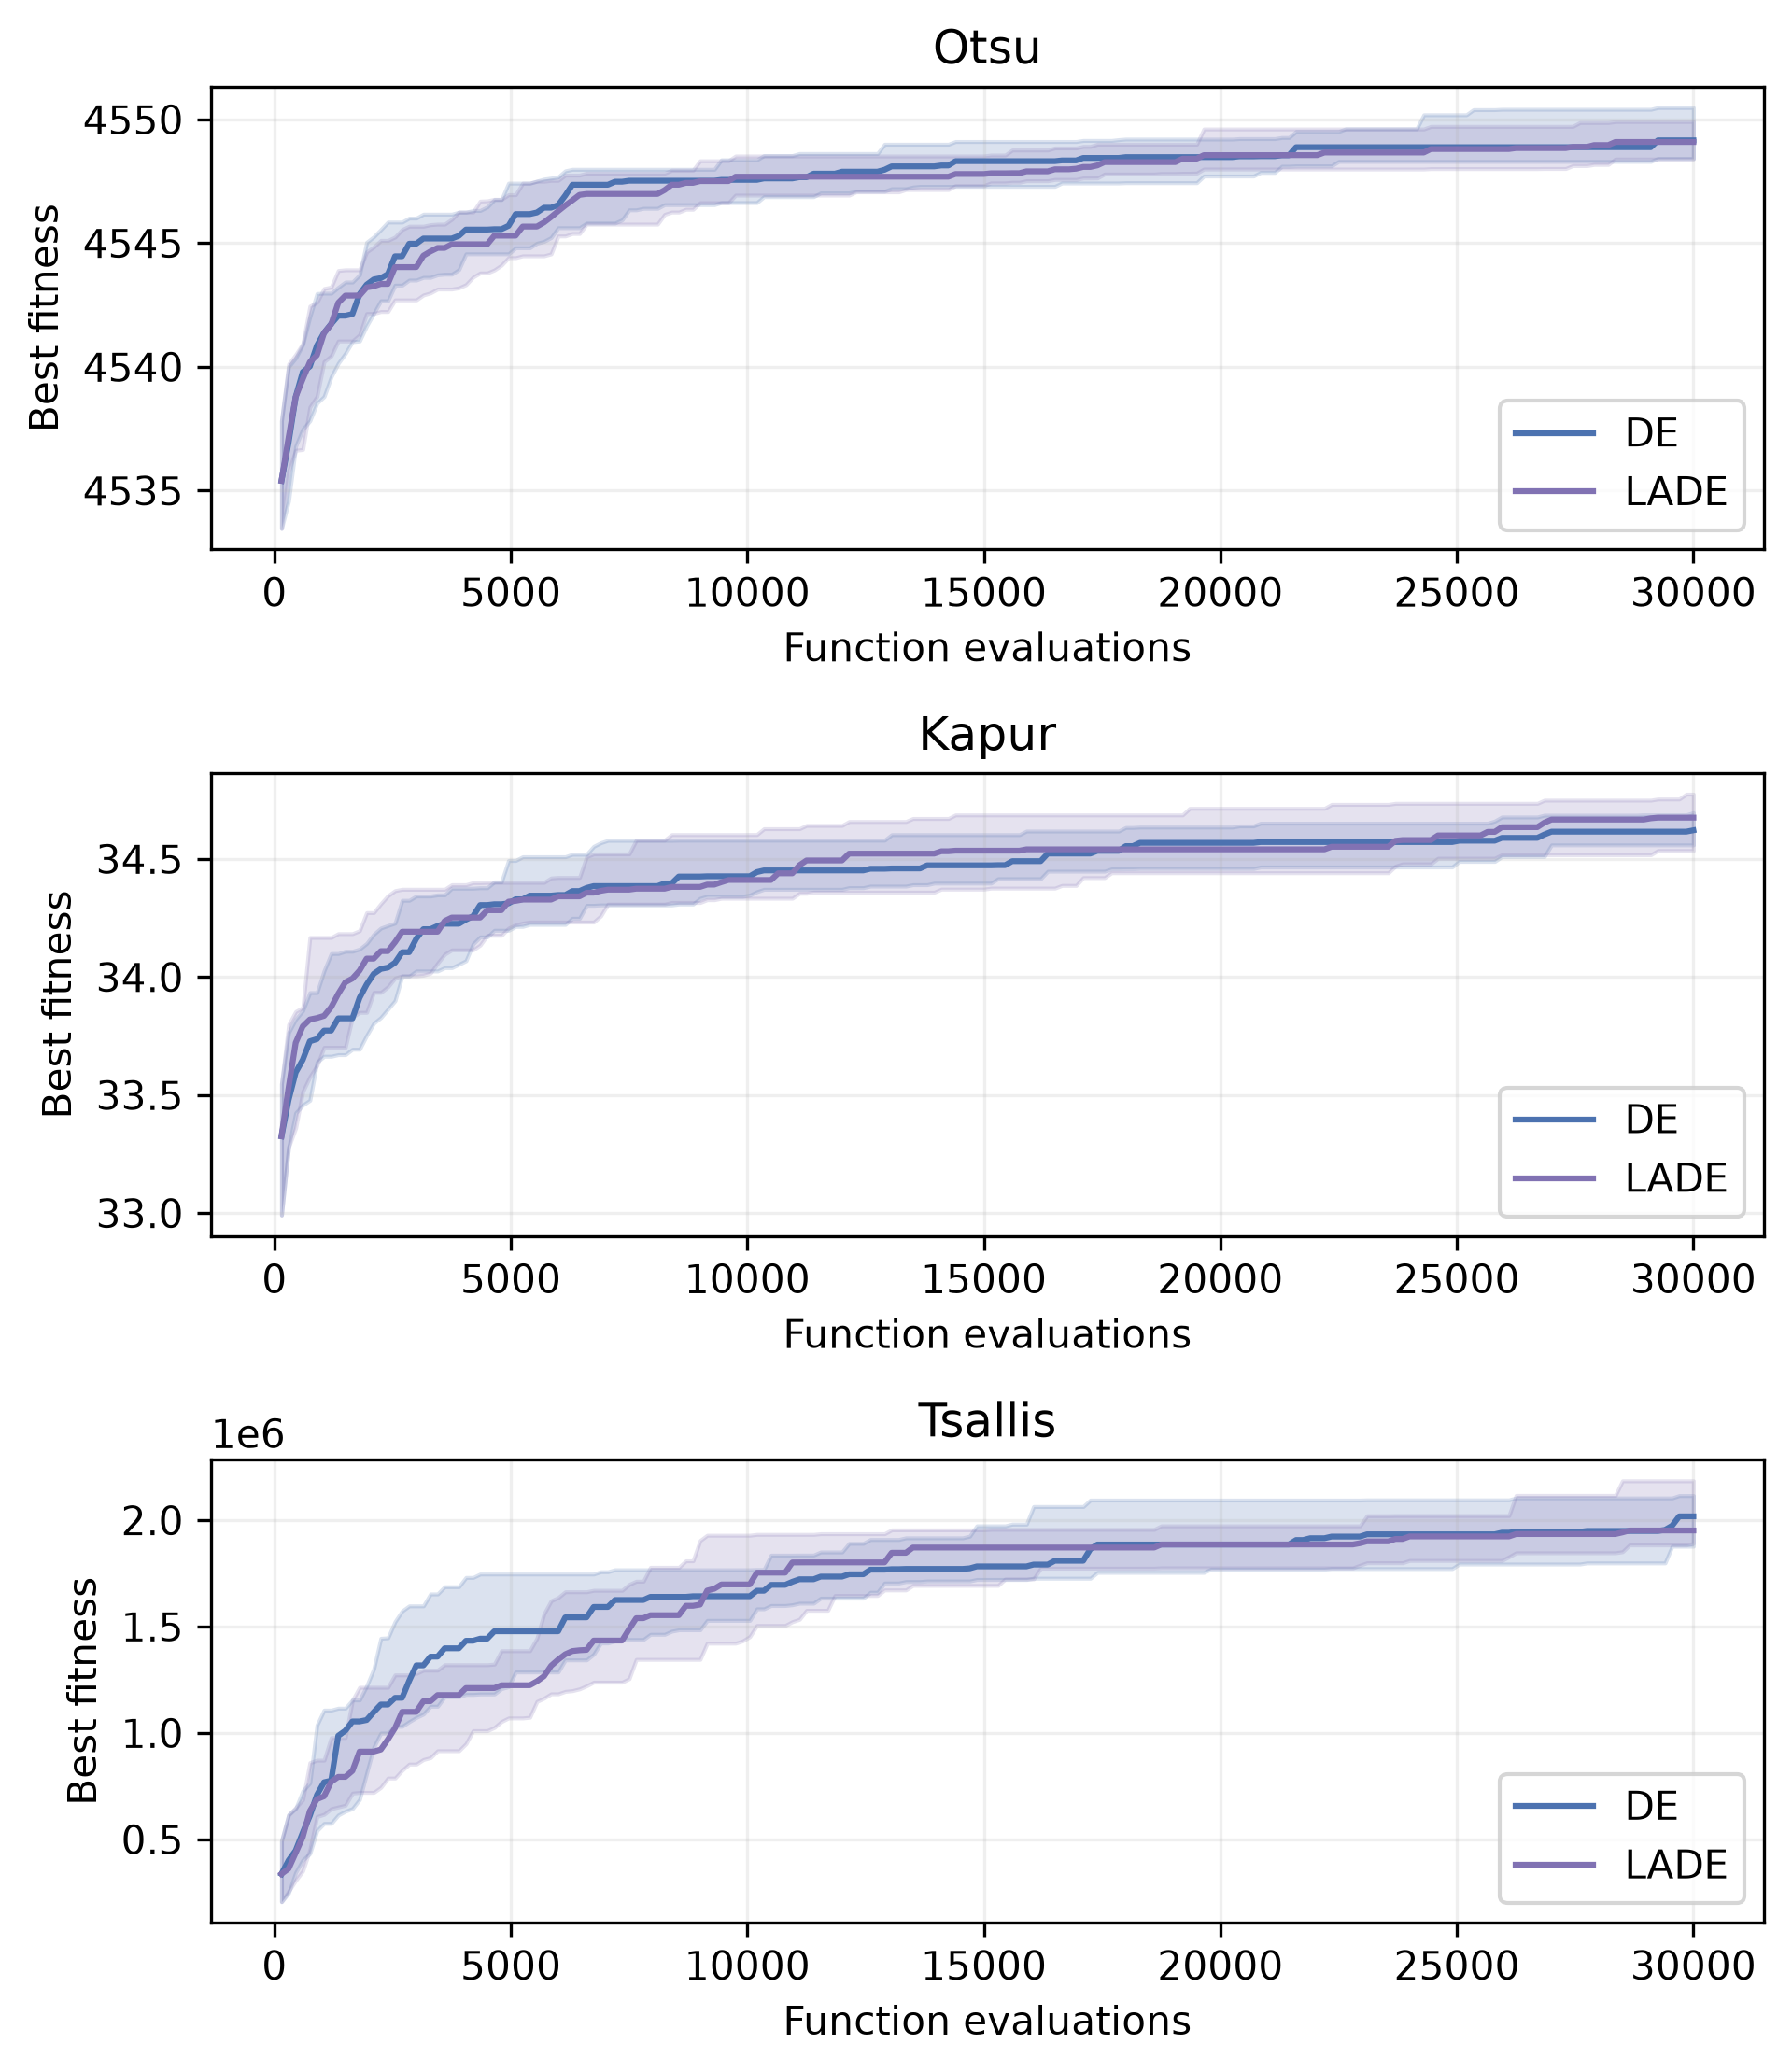
\includegraphics[width=\textwidth]{exp1_convergence.png}

\caption{Best-so-far fitness for img1 at $K=12$. Lines show the median over 30 runs and shaded bands show the interquartile range. Each panel uses its own objective scale; fitness values are not comparable across objectives.}

\label{fig:bsd_convergence}

\end{figure}

Figure~\ref{fig:bsd_convergence} compares convergence under an equal evaluation budget. Best-so-far fitness is retained independently of the current population in LADE, so its curves remain nondecreasing despite acceptance of some worse trials. These curves describe one illustrative image and do not alone establish a dataset-wide convergence advantage.

\subsubsection{Visual Segmentation Results}

\begin{figure}[htbp]

\centering

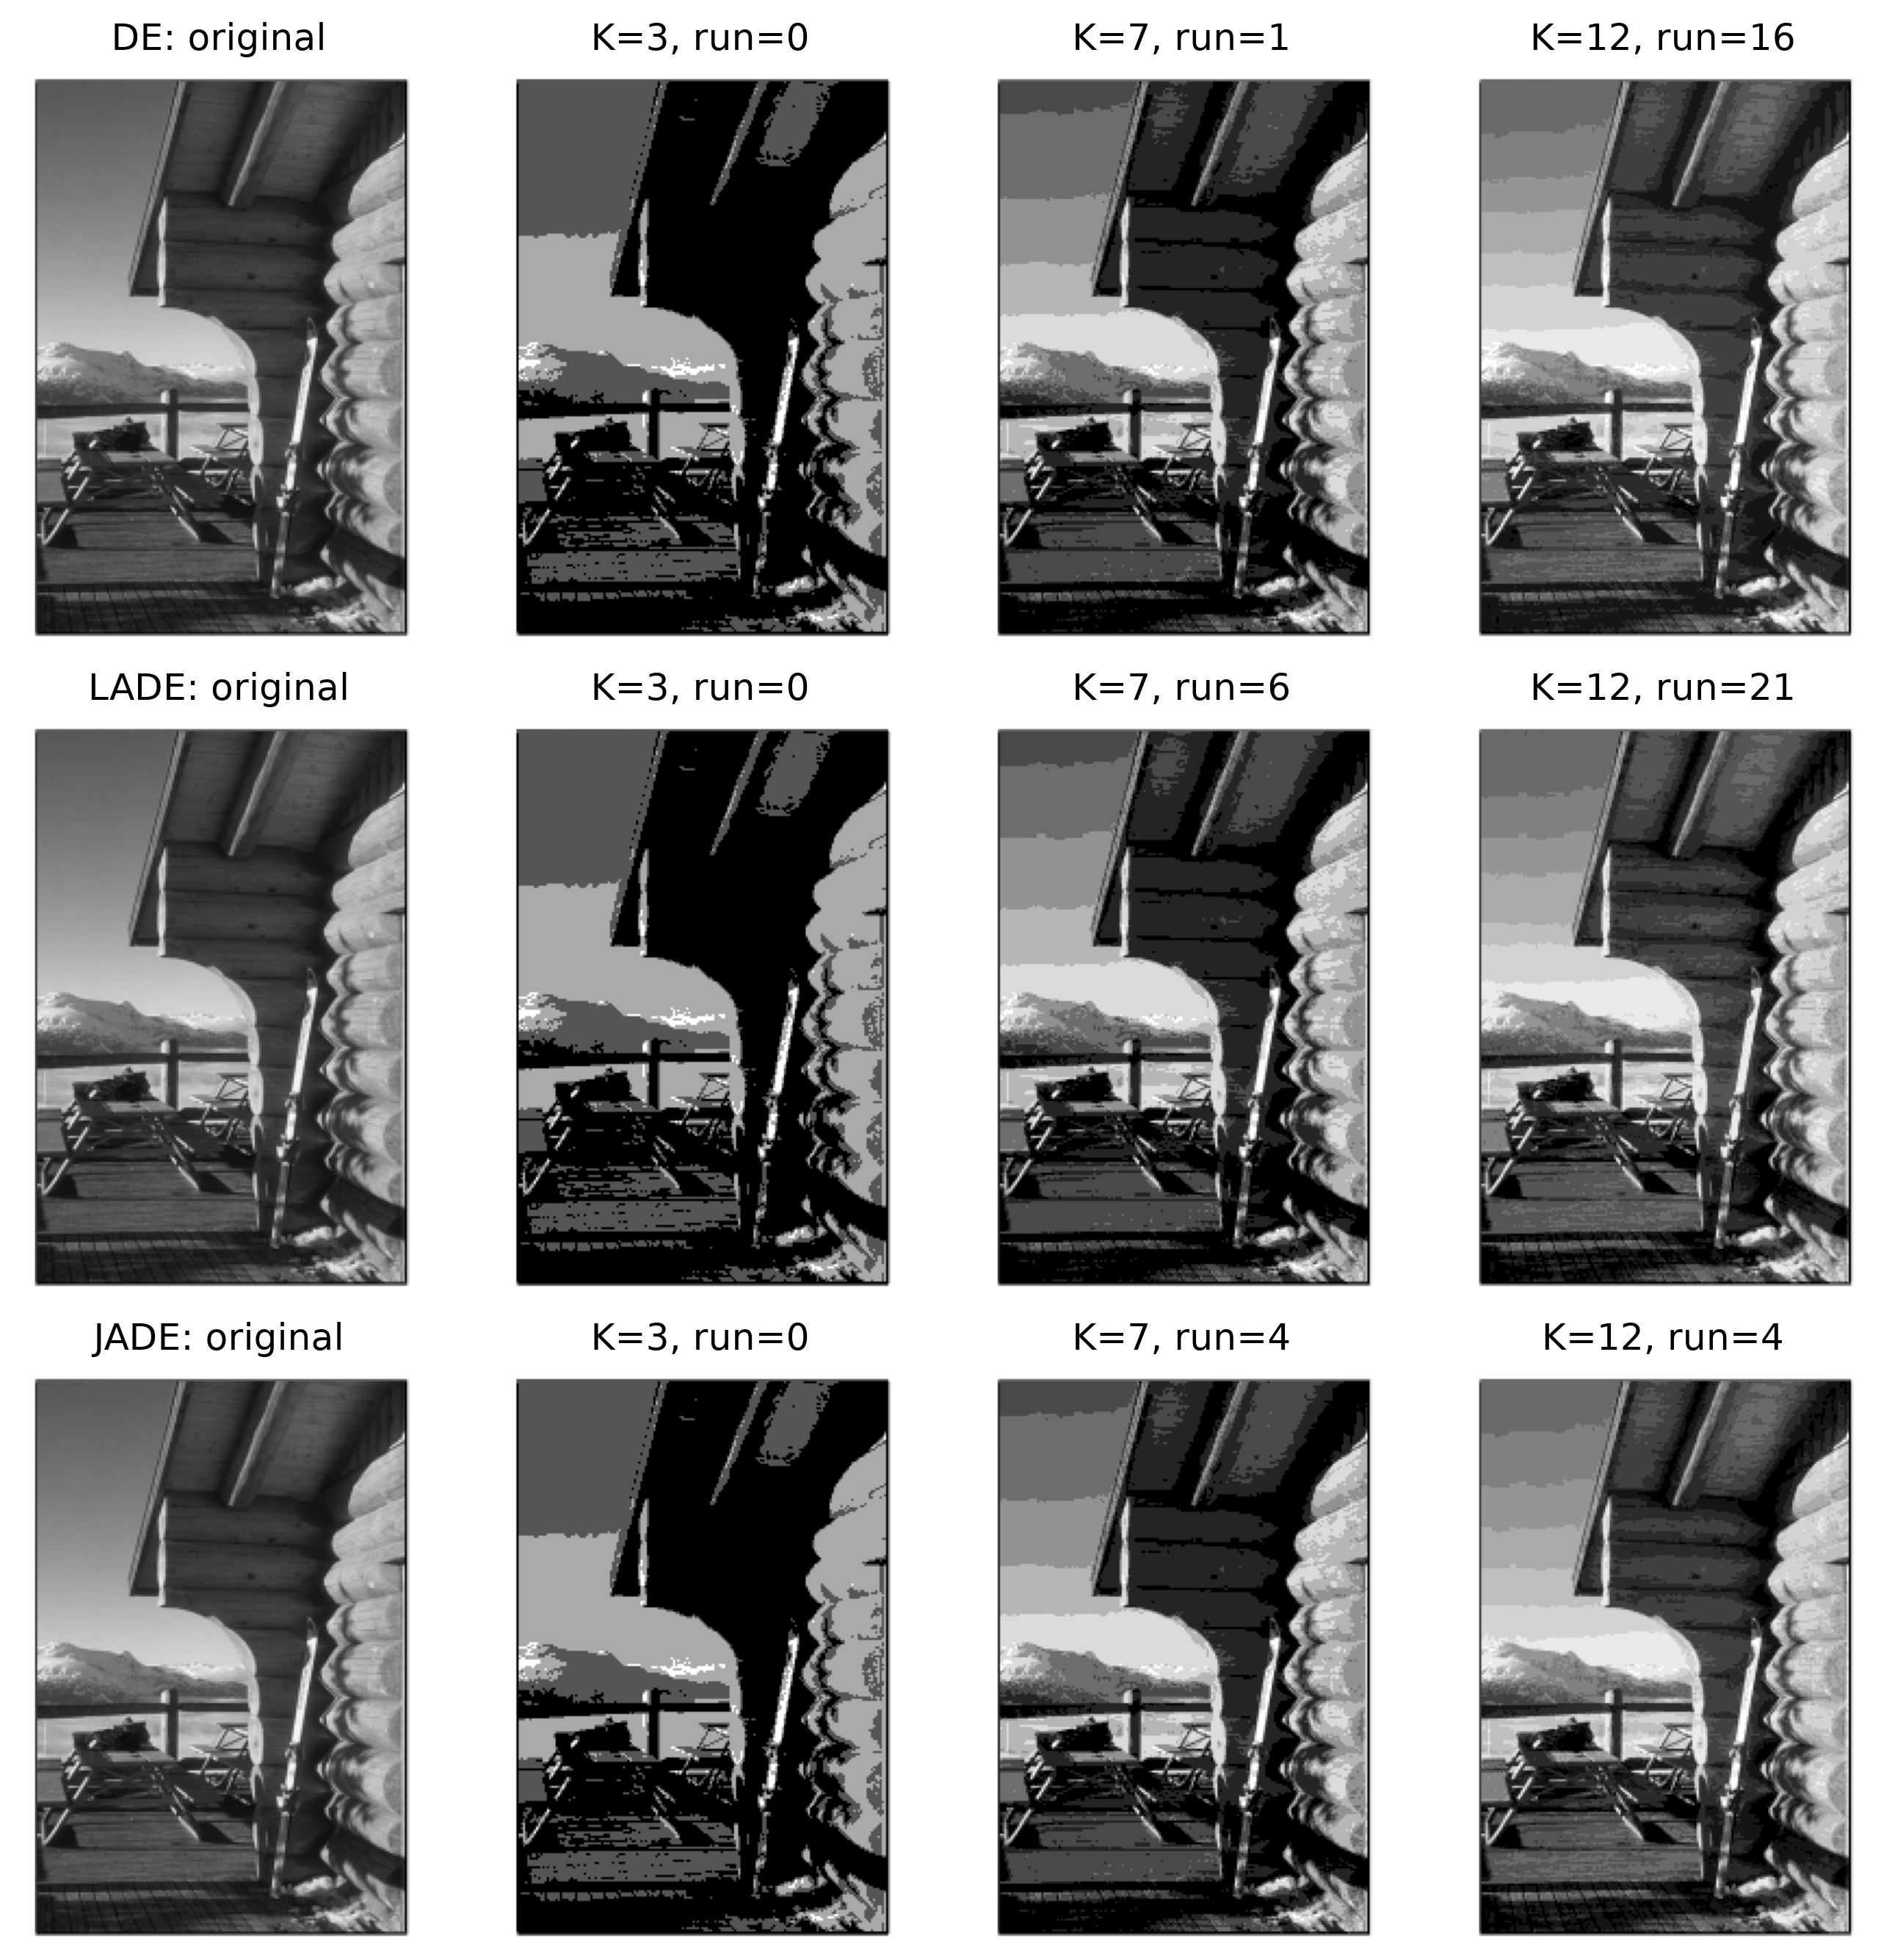
\includegraphics[width=0.9\textwidth]{exp1_segmentation_otsu.png}

\caption{Original and segmented img1 under Otsu at $K=3,7,12$. DE occupies the first row and LADE the second. Each solution is selected by fitness closest to the median of its 30 runs (ties use the lowest run index). Class intensities are spread evenly for display; PSNR and SSIM are computed using class means instead.}

\label{fig:bsd-segmentation-otsu}

\end{figure}

\begin{figure}[htbp]

\centering

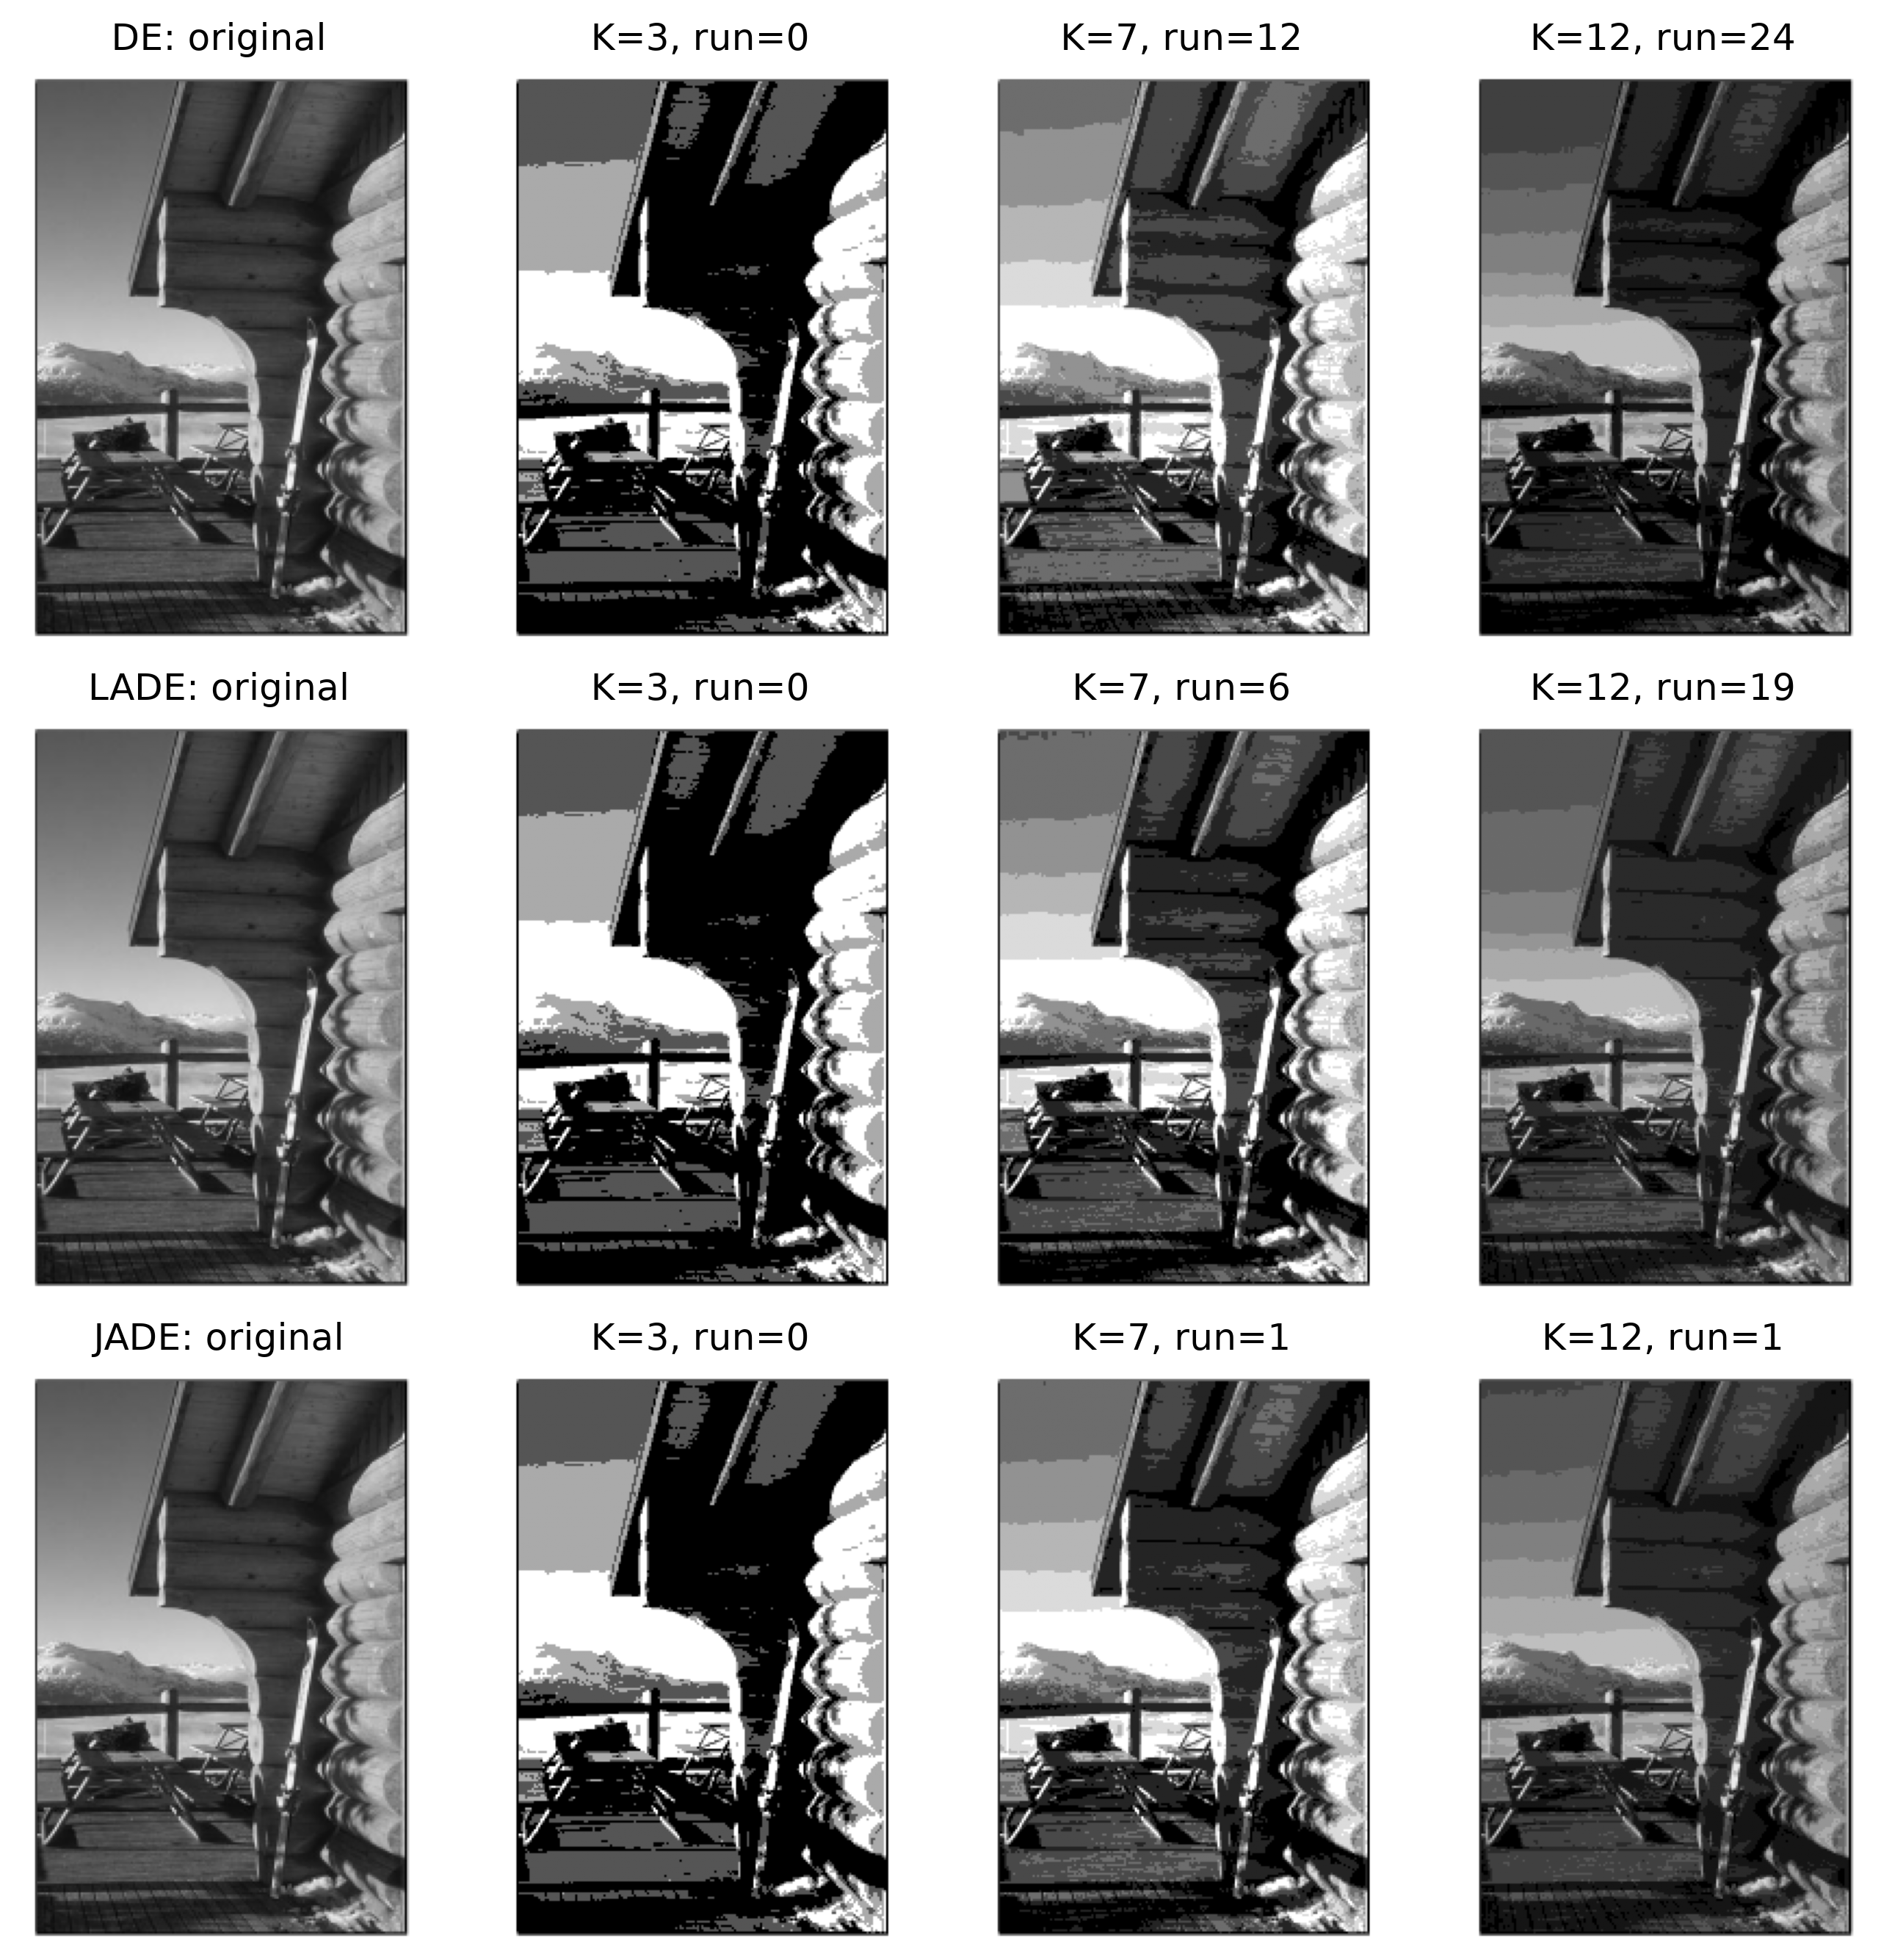
\includegraphics[width=0.9\textwidth]{exp1_segmentation_kapur.png}

\caption{Original and segmented img1 under Kapur at $K=3,7,12$. DE occupies the first row and LADE the second. Each solution is selected by fitness closest to the median of its 30 runs (ties use the lowest run index). Class intensities are spread evenly for display; PSNR and SSIM are computed using class means instead.}

\label{fig:bsd-segmentation-kapur}

\end{figure}

\begin{figure}[htbp]

\centering

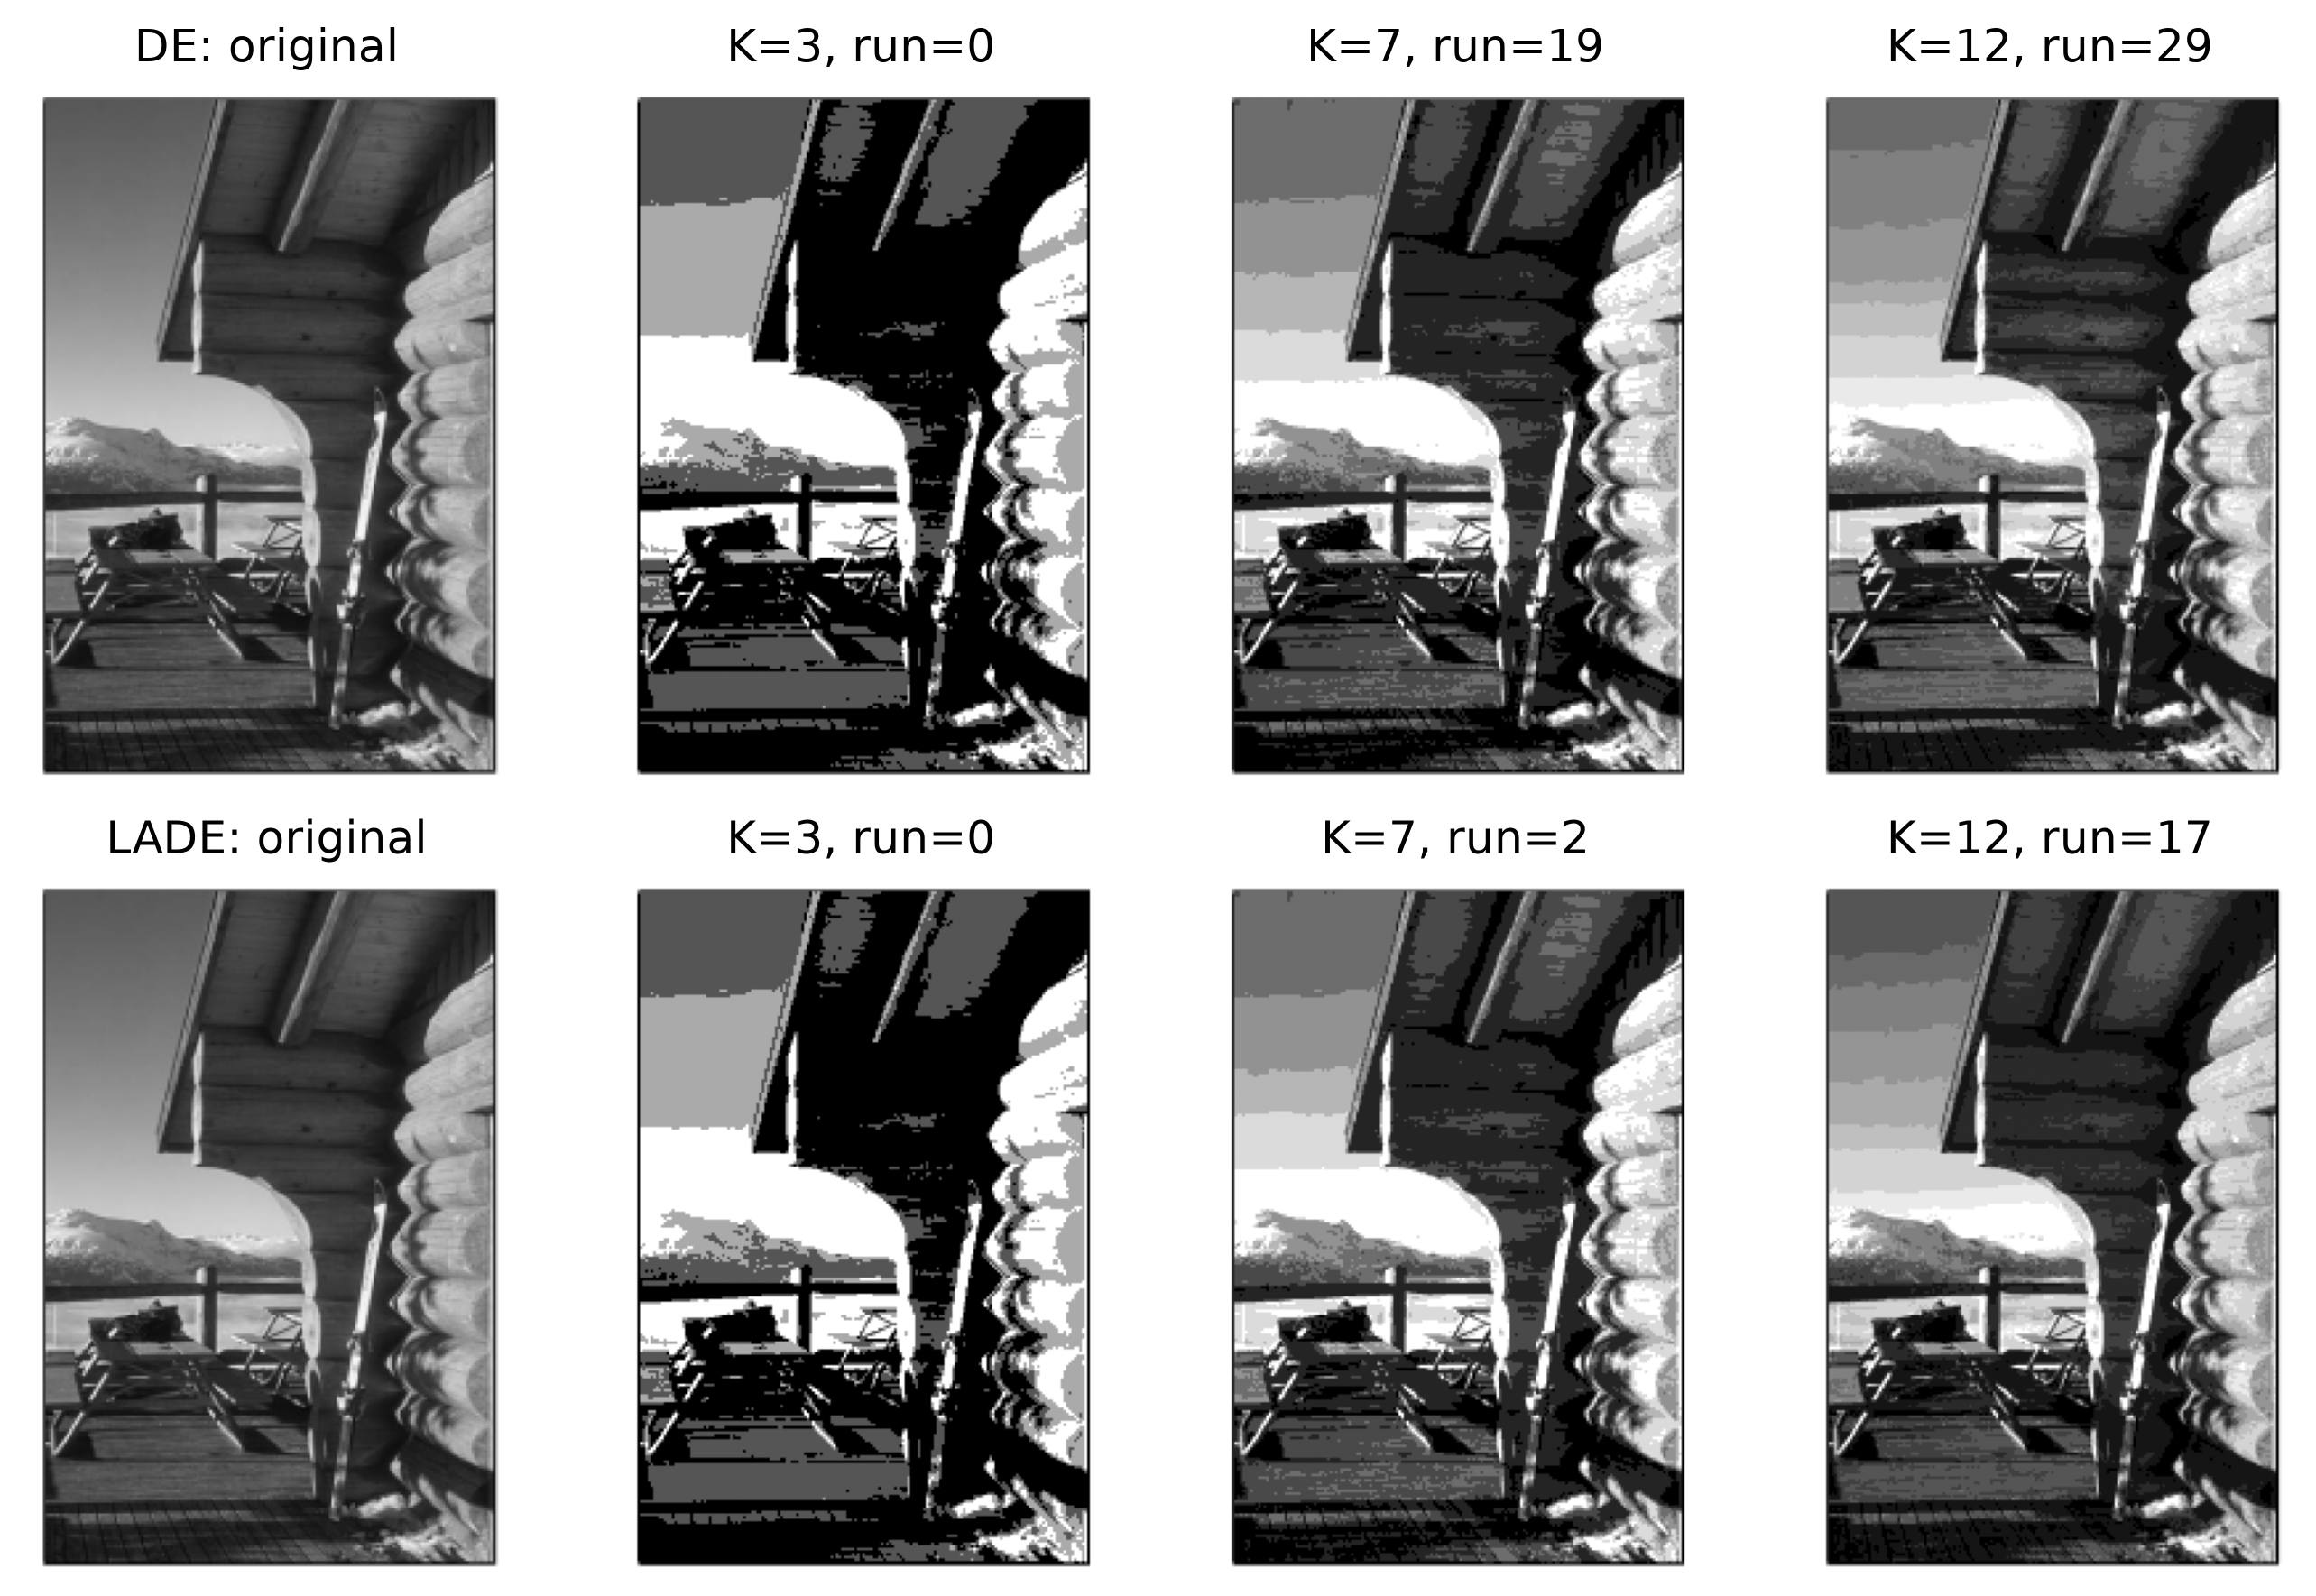
\includegraphics[width=0.9\textwidth]{exp1_segmentation_tsallis.png}

\caption{Original and segmented img1 under Tsallis at $K=3,7,12$. DE occupies the first row and LADE the second. Each solution is selected by fitness closest to the median of its 30 runs (ties use the lowest run index). Class intensities are spread evenly for display; PSNR and SSIM are computed using class means instead.}

\label{fig:bsd-segmentation-tsallis}

\end{figure}

\clearpage

\subsubsection{Execution Time}

\begin{figure}[htbp]

\centering

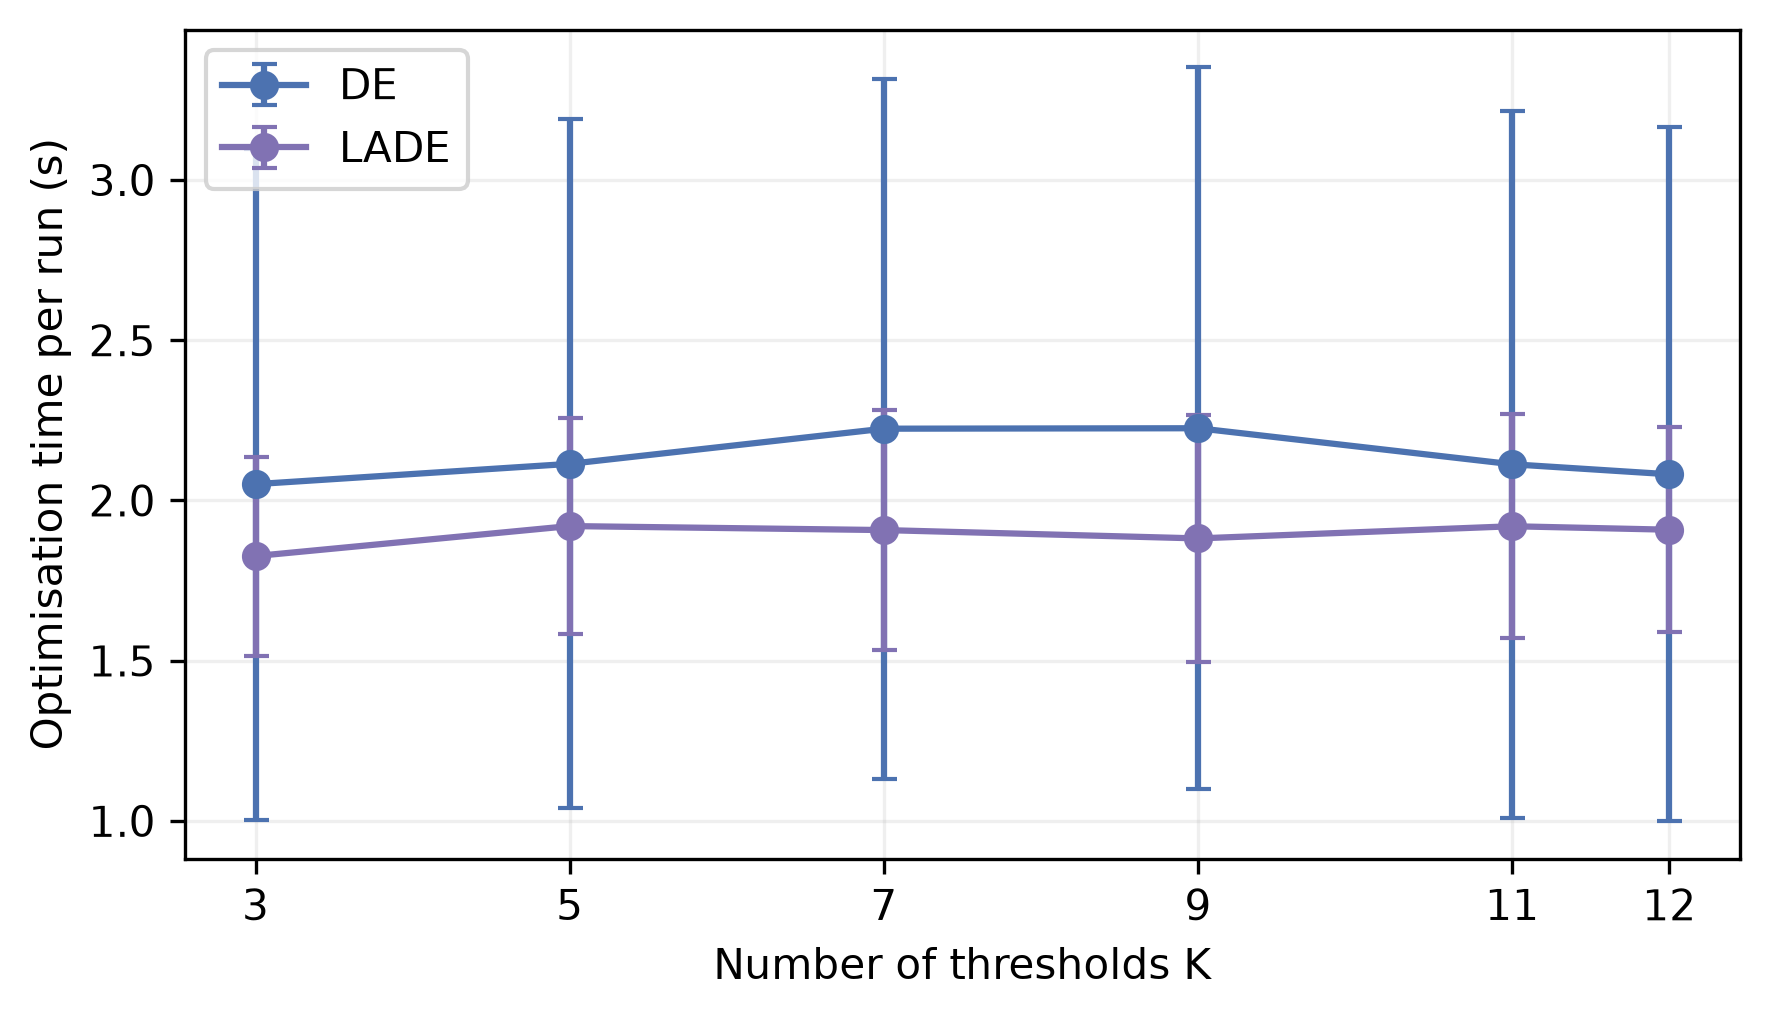
\includegraphics[width=0.8\textwidth]{exp1_runtime.png}

\caption{Mean recorded optimisation time versus $K$. Error bars show sample standard deviation over 900 runs per algorithm and threshold count (10 images, three objectives, 30 runs). DE and LADE were run in separate sweeps, so machine load and worker settings can influence this comparison.}

\label{fig:bsd-runtime}

\end{figure}

Timing covers optimiser execution and objective evaluations using \texttt{time.perf\_counter}; image loading, histogram preparation, exact reference computation, metric calculation and result writing are excluded. The saved results do not record hardware or worker counts, so runtime differences cannot be attributed exclusively to algorithm design.

\subsubsection{Discussion of Experiment 1}

Neither algorithm consistently dominates the reconstruction metrics. DE has slightly higher mean Otsu PSNR from $K=7$ through $K=12$, whereas LADE has higher mean Kapur PSNR at $K=5,9,11,12$. At $K=12$, LADE exceeds DE's Kapur PSNR by 0.1906 dB, while DE exceeds LADE's Otsu PSNR by 0.0406 dB. The Otsu results are identical at $K=3$. These small descriptive differences do not demonstrate significant superiority. LADE retains fixed DE control parameters and changes selection through a best-per-history-slot policy; this policy should be considered when interpreting the comparison. The experiment supports the expected improvement in reconstruction with more thresholds and shows a stronger descriptive effect of objective choice than of switching between these two optimisers. Full group conclusions require the remaining algorithms, paired statistical analysis and the MRI experiment.

\subsection{SHADE and L-SHADE with a Budget of 8{,}000 Function Evaluations}
\label{sec:shade-lshade}

\subsubsection{Experimental setting}

This subsection reports SHADE and L-SHADE on the same ten BSD500 images, the
same objectives (Otsu, Kapur, Tsallis with $q=0.8$) and the same values of
$K\in\{3,5,7,9,11,12\}$, using 30 independent runs per combination. Both
algorithms were given an identical budget of \textbf{8{,}000} function
evaluations (including initialisation), and the run with index $r$ used the
same random seed for both algorithms. SHADE used a population of 30
individuals and a history memory of $H=10$. L-SHADE started from
$N_{\text{init}}=\max(30,18K)$ individuals and reduced the population linearly
(as a function of consumed evaluations) to $N_{\min}=4$. Every run consumed
exactly 8{,}000 evaluations.

The budget used here (8{,}000 evaluations) differs from that of the DE and LADE
experiments (30{,}000 evaluations). The results in this subsection therefore
\emph{must not} be compared directly with Tables~2--10; they support only the
comparison between SHADE and L-SHADE.

In contrast to the pooled values reported for DE and LADE, each run's metric
is first averaged over the ten images, and the mean and sample standard
deviation are then computed over the 30 runs. The reported $\sigma$ therefore
measures run-to-run variability of the algorithm and excludes differences
between images.

\subsubsection{Reconstruction performance}

\begin{table}[htbp]
\centering
\small
\caption{SHADE on BSD500 (8{,}000 evaluations): mean $\pm$ standard deviation over 30 independent runs, each averaged over 10 images.}
\label{tab:shade-results}
\resizebox{\textwidth}{!}{%
\begin{tabular}{llcccccc}
\toprule
Metric & Objective & $K=3$ & $K=5$ & $K=7$ & $K=9$ & $K=11$ & $K=12$ \\
\midrule
\multirow{3}{*}{PSNR (dB)}
 & Otsu    & $27.97 \pm 0.00$ & $31.91 \pm 0.00$ & $34.75 \pm 0.01$ & $37.02 \pm 0.01$ & $38.72 \pm 0.02$ & $39.46 \pm 0.02$ \\
 & Kapur   & $23.66 \pm 0.00$ & $25.24 \pm 0.04$ & $27.73 \pm 0.33$ & $30.11 \pm 0.41$ & $32.56 \pm 0.40$ & $33.80 \pm 0.78$ \\
 & Tsallis & $23.73 \pm 0.00$ & $25.44 \pm 0.02$ & $27.10 \pm 0.08$ & $28.87 \pm 0.11$ & $29.79 \pm 0.11$ & $30.20 \pm 0.18$ \\
\midrule
\multirow{3}{*}{SSIM}
 & Otsu    & $0.8251 \pm 0.0000$ & $0.9073 \pm 0.0002$ & $0.9379 \pm 0.0004$ & $0.9544 \pm 0.0003$ & $0.9641 \pm 0.0005$ & $0.9685 \pm 0.0004$ \\
 & Kapur   & $0.8385 \pm 0.0006$ & $0.8839 \pm 0.0014$ & $0.9178 \pm 0.0017$ & $0.9306 \pm 0.0027$ & $0.9458 \pm 0.0027$ & $0.9527 \pm 0.0023$ \\
 & Tsallis & $0.8308 \pm 0.0002$ & $0.8821 \pm 0.0008$ & $0.9068 \pm 0.0010$ & $0.9258 \pm 0.0024$ & $0.9411 \pm 0.0019$ & $0.9474 \pm 0.0023$ \\
\midrule
\multirow{3}{*}{Uniformity}
 & Otsu    & $0.9862 \pm 0.0000$ & $0.9905 \pm 0.0000$ & $0.9928 \pm 0.0000$ & $0.9941 \pm 0.0000$ & $0.9950 \pm 0.0000$ & $0.9953 \pm 0.0000$ \\
 & Kapur   & $0.9636 \pm 0.0000$ & $0.9593 \pm 0.0003$ & $0.9705 \pm 0.0024$ & $0.9760 \pm 0.0015$ & $0.9820 \pm 0.0016$ & $0.9857 \pm 0.0031$ \\
 & Tsallis & $0.9654 \pm 0.0000$ & $0.9631 \pm 0.0003$ & $0.9660 \pm 0.0006$ & $0.9701 \pm 0.0008$ & $0.9699 \pm 0.0009$ & $0.9700 \pm 0.0013$ \\
\bottomrule
\end{tabular}%
}
\end{table}

\begin{table}[htbp]
\centering
\small
\caption{L-SHADE on BSD500 (8{,}000 evaluations): mean $\pm$ standard deviation over 30 independent runs, each averaged over 10 images.}
\label{tab:lshade-results}
\resizebox{\textwidth}{!}{%
\begin{tabular}{llcccccc}
\toprule
Metric & Objective & $K=3$ & $K=5$ & $K=7$ & $K=9$ & $K=11$ & $K=12$ \\
\midrule
\multirow{3}{*}{PSNR (dB)}
 & Otsu    & $27.97 \pm 0.00$ & $31.91 \pm 0.00$ & $34.74 \pm 0.01$ & $36.97 \pm 0.03$ & $38.55 \pm 0.04$ & $39.23 \pm 0.04$ \\
 & Kapur   & $23.66 \pm 0.00$ & $25.23 \pm 0.04$ & $27.74 \pm 0.17$ & $30.24 \pm 0.49$ & $32.56 \pm 0.41$ & $33.42 \pm 0.45$ \\
 & Tsallis & $23.73 \pm 0.00$ & $25.44 \pm 0.02$ & $27.13 \pm 0.07$ & $28.81 \pm 0.14$ & $29.77 \pm 0.14$ & $30.23 \pm 0.23$ \\
\midrule
\multirow{3}{*}{SSIM}
 & Otsu    & $0.8251 \pm 0.0000$ & $0.9073 \pm 0.0002$ & $0.9379 \pm 0.0003$ & $0.9539 \pm 0.0005$ & $0.9633 \pm 0.0006$ & $0.9675 \pm 0.0006$ \\
 & Kapur   & $0.8386 \pm 0.0004$ & $0.8837 \pm 0.0014$ & $0.9180 \pm 0.0017$ & $0.9310 \pm 0.0028$ & $0.9449 \pm 0.0026$ & $0.9519 \pm 0.0025$ \\
 & Tsallis & $0.8308 \pm 0.0001$ & $0.8822 \pm 0.0006$ & $0.9070 \pm 0.0015$ & $0.9251 \pm 0.0024$ & $0.9416 \pm 0.0031$ & $0.9468 \pm 0.0029$ \\
\midrule
\multirow{3}{*}{Uniformity}
 & Otsu    & $0.9862 \pm 0.0000$ & $0.9905 \pm 0.0000$ & $0.9927 \pm 0.0000$ & $0.9941 \pm 0.0000$ & $0.9948 \pm 0.0000$ & $0.9951 \pm 0.0000$ \\
 & Kapur   & $0.9636 \pm 0.0000$ & $0.9591 \pm 0.0003$ & $0.9708 \pm 0.0005$ & $0.9764 \pm 0.0016$ & $0.9821 \pm 0.0017$ & $0.9843 \pm 0.0020$ \\
 & Tsallis & $0.9654 \pm 0.0000$ & $0.9631 \pm 0.0003$ & $0.9662 \pm 0.0006$ & $0.9696 \pm 0.0012$ & $0.9698 \pm 0.0009$ & $0.9705 \pm 0.0018$ \\
\bottomrule
\end{tabular}%
}
\end{table}

\begin{table}[htbp]
\centering
\small
\caption{Execution time (seconds per run, 8{,}000 evaluations): mean $\pm$ standard deviation over all runs, images and objectives.}
\label{tab:shade-lshade-time}
\resizebox{\textwidth}{!}{%
\begin{tabular}{lcccccc}
\toprule
Algorithm & $K=3$ & $K=5$ & $K=7$ & $K=9$ & $K=11$ & $K=12$ \\
\midrule
SHADE   & $0.95 \pm 0.62$ & $0.93 \pm 0.64$ & $0.91 \pm 0.59$ & $0.94 \pm 0.59$ & $0.92 \pm 0.58$ & $0.97 \pm 0.64$ \\
L-SHADE & $0.94 \pm 0.65$ & $0.98 \pm 0.65$ & $1.04 \pm 0.78$ & $1.13 \pm 0.85$ & $1.15 \pm 0.80$ & $1.14 \pm 0.81$ \\
\bottomrule
\end{tabular}%
}
\end{table}

\subsubsection{Effect of the number of thresholds}

For both algorithms and all three objectives, PSNR and SSIM increase with
$K$, as expected when more classes are available to approximate the image. The
largest PSNR gain between $K=3$ and $K=12$ occurs for Otsu (SHADE: $+11.49$~dB,
from 27.97 to 39.46~dB), followed by Kapur ($+10.14$~dB) and Tsallis
($+6.47$~dB). The gains diminish with $K$: for SHADE with Otsu, moving from
$K=3$ to $K=5$ adds 3.94~dB, whereas moving from $K=11$ to $K=12$ adds only
0.74~dB. Uniformity is not strictly monotonic for the entropy-based
objectives: it falls slightly between $K=3$ and $K=5$ for both Kapur (0.9636
to 0.9593 for SHADE) and Tsallis (0.9654 to 0.9631), and the metric contains
an explicit factor of $K$, so a larger PSNR does not guarantee a larger
Uniformity score.

\subsubsection{Otsu versus Kapur versus Tsallis ($q=0.8$)}

 
Otsu yields the highest PSNR and Uniformity at every $K$. For SHADE the margin
over Kapur in PSNR is 4.31~dB at $K=3$ and 5.66~dB at $K=12$. This ordering is
expected from the reconstruction rule. Because each pixel is replaced by its
class mean, the mean squared error equals the total image variance minus the
between-class variance, which is exactly the quantity maximised by Otsu's
criterion. The globally optimal Otsu thresholds therefore minimise the
reconstruction error for a given $K$ and act as an upper bound on the PSNR of
the other two objectives. Uniformity is built from the within-class scatter
and shows the same ordering.

At small $K$ the two entropy-based criteria are close, with Tsallis marginally
ahead in PSNR at $K=3$ (23.73 versus 23.66~dB) and $K=5$ (25.44 versus
25.24~dB). From $K=7$ onwards Kapur is clearly better, and the gap widens to
3.60~dB at $K=12$ (33.80 versus 30.20~dB). The Uniformity of Tsallis stays
near 0.97 for $K\geq 7$, while that of Kapur keeps rising (0.9857 at $K=12$),
so the Tsallis objective with $q=0.8$ appears to saturate earlier as the
number of classes grows.

The ranking of the objectives depends on the metric. At $K=3$ Kapur attains
the highest SSIM (0.8385), followed by Tsallis (0.8308) and Otsu (0.8251),
although it has the lowest PSNR. From $K=5$ onward Otsu has the highest SSIM.
Hence the entropy-based criteria can preserve local structure at small $K$
despite a larger squared error. Only $q=0.8$ was evaluated, so these results
describe the Tsallis objective at this value and do not characterise the
general influence of the non-extensive parameter $q$.

\subsubsection{Reliability of the optimisation}

The run-to-run standard deviation indicates how hard each landscape is for
the optimisers. For Otsu it is negligible (at most 0.04~dB in PSNR and 0.0006
in SSIM), so both algorithms reach essentially the same solution in every run.
Tsallis shows small variability (at most 0.23~dB), whereas Kapur is the least
consistent, with a standard deviation of up to 0.78~dB at $K=12$, which
suggests a more multimodal landscape. Differences between the algorithms are
therefore most likely to appear on Kapur at large $K$.

\subsubsection{SHADE versus L-SHADE}

The two algorithms perform very similarly. For $K\leq 7$ (all objectives) and
for Tsallis at every $K$, the PSNR differences are at most 0.06~dB and lie
well inside the run-to-run variability. Small but systematic differences occur
for Otsu at large $K$, where SHADE is ahead by 0.05~dB at $K=9$, 0.17~dB at
$K=11$ and 0.23~dB at $K=12$; the same ordering is seen in SSIM (0.9685
versus 0.9675 at $K=12$). For Kapur, L-SHADE is ahead at $K=9$ ($+0.13$~dB) and
behind at $K=12$ ($-0.38$~dB), but both differences are within the spread of
the runs (0.4 to 0.8~dB), so no consistent winner emerges. L-SHADE is more
stable than SHADE on Kapur at $K=7$ (standard deviation 0.17 versus 0.33~dB).

A plausible reason for the small disadvantage of L-SHADE on Otsu at large $K$
is its initial population of $18K$ individuals (216 at $K=12$): with only
8{,}000 evaluations this leaves roughly 37 generations before the population
is reduced to its minimum size, which may prevent full convergence. This
explanation is a hypothesis; it was not tested by varying $N_{\text{init}}$.

\subsubsection{Convergence behaviour}

Figure~\ref{fig:convergence} shows the mean best fitness against the number of
function evaluations for image \texttt{IMG}, averaged over the 30 runs, for
each value of $K$ and each objective. Both algorithms use the same budget of
8{,}000 evaluations, so the curves share a common horizontal axis even though
the population sizes differ (SHADE: 30; L-SHADE: $\max(30,18K)$ reducing to 4).
Fitness values are not comparable across objectives, since each objective has
its own scale.
\begin{figure}[htbp] 
  \centering
  \begin{subfigure}{\textwidth}
    \centering
    \includegraphics[width=\textwidth]{convergence_img1_gt_otsu.png}
    \caption{Otsu}
  \end{subfigure}
  
\medskip
  \begin{subfigure}{\textwidth}
    \centering
    \includegraphics[width=\textwidth]{segmentation_img1_gt_otsu.png}
    \caption{Image 1}
  \end{subfigure}
  
  \caption{Convergence of SHADE and L-SHADE on image \texttt{Image 1}: mean best
  fitness over 30 runs versus function evaluations, for $K\in\{3,5,7,9,11,12\}$.}
  \label{fig:convergence}
\end{figure}


\subsubsection{Execution time}
SHADE requires about 0.9 to 1.0~s per run irrespective of $K$, because the
fixed budget of 8{,}000 evaluations dominates the cost
(Table~\ref{tab:shade-lshade-time}). The run time of L-SHADE increases from
0.94~s at $K=3$ to 1.14~s at $K=12$, up to about 25\% more than SHADE at the
largest $K$. Both algorithms use the same number of evaluations, so the
difference reflects algorithmic overhead, which grows with the larger initial
population (sorting, archive maintenance and population reduction). The
standard deviations are large (0.6 to 0.8~s) because they pool all
objectives and images and the runs shared CPU cores. The timing trend should
therefore be regarded as indicative and not as a precise benchmark.

\subsubsection{Limitations}

This subsection compares only SHADE and L-SHADE at a single budget of 8{,}000
evaluations, a single value of $q$ and ten BSD500 images. It does not show
whether either algorithm outperforms DE or LADE, because those experiments
used a different budget. The conclusions should be confirmed on a larger image
set before being generalised.


\section{Experiment 2: CHAOS MRI Images}
\label{sec:experiment2}
\subsection{Experimental Objective and Available Data}

This experiment evaluates the completed DE and LADE implementations on the
15 supplied CHAOS abdominal MRI slices. Each algorithm was evaluated with
Otsu, Kapur and Tsallis ($q=0.8$) at
$K\in\{3,5,7,9,11,12\}$, using 30 runs per combination and the same
30,000-evaluation budget as Experiment~1. This gives 2,700 runs per
algorithm and 5,400 runs in total.

Only the MRI slices, named \texttt{IMG-*.png}, are present in the supplied
\texttt{data/CHAOS/} directory. No anatomical ground-truth masks are
available. Consequently, Dice and Jaccard scores, and automatic matching of
threshold classes to a target organ, cannot be computed from this dataset.
Reporting either score without masks would not constitute a ground-truth
segmentation evaluation. The experiment therefore reports reconstruction
quality and unsupervised class separability.

Each table entry below pools 450 observations (15 images and 30 independent
runs per image) and reports the pooled mean and sample standard deviation.
The standard deviations therefore combine between-image variation with
within-image stochastic variation and should not be interpreted solely as
algorithmic instability. Results for JADE, SHADE and L-SHADE are pending and
are not included.

\subsection{Reconstruction and Separability Results}

\begin{table}[htbp]
\centering
\small
\caption{PSNR (dB) on CHAOS: pooled mean $\pm$ sample standard deviation across 450 observations per entry.}
\label{tab:chaos-psnr}
\resizebox{\textwidth}{!}{%
\begin{tabular}{llcccccc}
\toprule
Objective & Algorithm & $K=3$ & $K=5$ & $K=7$ & $K=9$ & $K=11$ & $K=12$ \\
\midrule
Otsu & DE & $27.8831 \pm 0.8927$ & $31.4138 \pm 0.8965$ & $33.8331 \pm 0.9564$ & $35.3458 \pm 0.9609$ & $36.5615 \pm 0.9729$ & $37.1370 \pm 0.9576$ \\
Otsu & LADE & $27.8831 \pm 0.8927$ & $31.4138 \pm 0.8965$ & $33.7570 \pm 0.9526$ & $35.2925 \pm 0.9638$ & $36.5373 \pm 0.9430$ & $37.1047 \pm 0.9660$ \\
Kapur & DE & $23.9217 \pm 3.2645$ & $29.5546 \pm 1.0739$ & $32.5833 \pm 0.8853$ & $34.2965 \pm 0.9654$ & $35.5513 \pm 1.0270$ & $36.1433 \pm 0.9929$ \\
Kapur & LADE & $23.9227 \pm 3.2664$ & $29.5522 \pm 1.0768$ & $32.5398 \pm 0.8799$ & $34.2192 \pm 0.9770$ & $35.5391 \pm 0.9809$ & $36.1674 \pm 1.0023$ \\
Tsallis & DE & $19.2215 \pm 1.6472$ & $21.6107 \pm 1.1139$ & $23.3961 \pm 1.3927$ & $25.6068 \pm 2.0485$ & $30.6101 \pm 3.6384$ & $32.5967 \pm 3.4584$ \\
Tsallis & LADE & $19.2181 \pm 1.6513$ & $21.6014 \pm 1.1181$ & $23.3535 \pm 1.4040$ & $25.7208 \pm 2.1794$ & $30.5670 \pm 3.6296$ & $32.6407 \pm 3.6075$ \\
\bottomrule
\end{tabular}%
}
\end{table}

\begin{table}[htbp]
\centering
\small
\caption{SSIM on CHAOS: pooled mean $\pm$ sample standard deviation across 450 observations per entry.}
\label{tab:chaos-ssim}
\resizebox{\textwidth}{!}{%
\begin{tabular}{llcccccc}
\toprule
Objective & Algorithm & $K=3$ & $K=5$ & $K=7$ & $K=9$ & $K=11$ & $K=12$ \\
\midrule
Otsu & DE & $0.8664 \pm 0.0411$ & $0.9242 \pm 0.0220$ & $0.9495 \pm 0.0146$ & $0.9612 \pm 0.0120$ & $0.9691 \pm 0.0097$ & $0.9721 \pm 0.0090$ \\
Otsu & LADE & $0.8664 \pm 0.0411$ & $0.9243 \pm 0.0220$ & $0.9487 \pm 0.0150$ & $0.9607 \pm 0.0122$ & $0.9688 \pm 0.0098$ & $0.9718 \pm 0.0089$ \\
Kapur & DE & $0.6508 \pm 0.2917$ & $0.9107 \pm 0.0267$ & $0.9398 \pm 0.0166$ & $0.9537 \pm 0.0136$ & $0.9625 \pm 0.0118$ & $0.9662 \pm 0.0106$ \\
Kapur & LADE & $0.6509 \pm 0.2916$ & $0.9107 \pm 0.0268$ & $0.9395 \pm 0.0164$ & $0.9532 \pm 0.0139$ & $0.9625 \pm 0.0117$ & $0.9662 \pm 0.0108$ \\
Tsallis & DE & $0.2651 \pm 0.0369$ & $0.3339 \pm 0.0454$ & $0.3942 \pm 0.0607$ & $0.4913 \pm 0.1030$ & $0.7339 \pm 0.1884$ & $0.8163 \pm 0.1675$ \\
Tsallis & LADE & $0.2650 \pm 0.0370$ & $0.3337 \pm 0.0457$ & $0.3926 \pm 0.0598$ & $0.4968 \pm 0.1153$ & $0.7298 \pm 0.1886$ & $0.8167 \pm 0.1745$ \\
\bottomrule
\end{tabular}%
}
\end{table}

\begin{table}[htbp]
\centering
\small
\caption{Uniformity on CHAOS: pooled mean $\pm$ sample standard deviation across 450 observations per entry.}
\label{tab:chaos-uniformity}
\resizebox{\textwidth}{!}{%
\begin{tabular}{llcccccc}
\toprule
Objective & Algorithm & $K=3$ & $K=5$ & $K=7$ & $K=9$ & $K=11$ & $K=12$ \\
\midrule
Otsu & DE & $0.9900 \pm 0.0020$ & $0.9926 \pm 0.0015$ & $0.9941 \pm 0.0012$ & $0.9946 \pm 0.0011$ & $0.9950 \pm 0.0010$ & $0.9953 \pm 0.0010$ \\
Otsu & LADE & $0.9900 \pm 0.0020$ & $0.9926 \pm 0.0015$ & $0.9940 \pm 0.0012$ & $0.9946 \pm 0.0011$ & $0.9950 \pm 0.0010$ & $0.9952 \pm 0.0010$ \\
Kapur & DE & $0.9654 \pm 0.0376$ & $0.9886 \pm 0.0031$ & $0.9921 \pm 0.0016$ & $0.9931 \pm 0.0015$ & $0.9937 \pm 0.0015$ & $0.9940 \pm 0.0014$ \\
Kapur & LADE & $0.9654 \pm 0.0376$ & $0.9885 \pm 0.0031$ & $0.9920 \pm 0.0016$ & $0.9930 \pm 0.0016$ & $0.9937 \pm 0.0014$ & $0.9940 \pm 0.0014$ \\
Tsallis & DE & $0.9225 \pm 0.0328$ & $0.9287 \pm 0.0184$ & $0.9326 \pm 0.0219$ & $0.9449 \pm 0.0258$ & $0.9728 \pm 0.0247$ & $0.9813 \pm 0.0185$ \\
Tsallis & LADE & $0.9224 \pm 0.0329$ & $0.9285 \pm 0.0184$ & $0.9318 \pm 0.0227$ & $0.9458 \pm 0.0258$ & $0.9730 \pm 0.0227$ & $0.9809 \pm 0.0193$ \\
\bottomrule
\end{tabular}%
}
\end{table}

\begin{table}[htbp]
\centering
\small
\caption{Class separability on CHAOS: pooled mean $\pm$ sample standard deviation across 450 observations per entry.}
\label{tab:chaos-class-separability}
\resizebox{\textwidth}{!}{%
\begin{tabular}{llcccccc}
\toprule
Objective & Algorithm & $K=3$ & $K=5$ & $K=7$ & $K=9$ & $K=11$ & $K=12$ \\
\midrule
Otsu & DE & $0.9760 \pm 0.0076$ & $0.9894 \pm 0.0030$ & $0.9940 \pm 0.0016$ & $0.9957 \pm 0.0011$ & $0.9968 \pm 0.0008$ & $0.9972 \pm 0.0007$ \\
Otsu & LADE & $0.9760 \pm 0.0076$ & $0.9894 \pm 0.0030$ & $0.9939 \pm 0.0016$ & $0.9957 \pm 0.0011$ & $0.9968 \pm 0.0008$ & $0.9972 \pm 0.0007$ \\
Kapur & DE & $0.9105 \pm 0.0956$ & $0.9836 \pm 0.0056$ & $0.9919 \pm 0.0024$ & $0.9945 \pm 0.0016$ & $0.9959 \pm 0.0013$ & $0.9964 \pm 0.0012$ \\
Kapur & LADE & $0.9104 \pm 0.0959$ & $0.9835 \pm 0.0056$ & $0.9918 \pm 0.0023$ & $0.9944 \pm 0.0018$ & $0.9959 \pm 0.0013$ & $0.9964 \pm 0.0011$ \\
Tsallis & DE & $0.8130 \pm 0.0917$ & $0.8968 \pm 0.0393$ & $0.9292 \pm 0.0325$ & $0.9553 \pm 0.0240$ & $0.9804 \pm 0.0202$ & $0.9868 \pm 0.0166$ \\
Tsallis & LADE & $0.8128 \pm 0.0919$ & $0.8963 \pm 0.0406$ & $0.9286 \pm 0.0324$ & $0.9558 \pm 0.0240$ & $0.9801 \pm 0.0202$ & $0.9864 \pm 0.0170$ \\
\bottomrule
\end{tabular}%
}
\end{table}

\subsection{Discussion of Experiment 2}

Increasing $K$ improves all four pooled metrics for both algorithms under
each objective. Otsu is the strongest objective descriptively at every
tested $K$. For example, DE at $K=12$ obtains mean PSNR values of
37.1370 dB with Otsu, 36.1433 dB with Kapur and 32.5967 dB with Tsallis.
The corresponding mean SSIM values are 0.9721, 0.9662 and 0.8163.
Tsallis improves sharply between $K=9$ and $K=12$, but remains below Otsu
and Kapur and exhibits substantially greater pooled variability at the
largest threshold counts. Only $q=0.8$ was evaluated, so the effect of
changing the Tsallis entropic index cannot be inferred.

DE and LADE produce very similar pooled results. Their Otsu results are
identical at $K=3$ and effectively identical at $K=5$; the largest displayed
Otsu PSNR difference is 0.0762 dB at $K=7$, in favour of DE. LADE is higher
on mean Kapur PSNR at $K=3$ and $K=12$, and on mean Tsallis PSNR at $K=9$
and $K=12$, but these descriptive differences are small relative to the
pooled standard deviations. Statistical testing is required before claiming
an algorithmic advantage. In contrast, objective choice and threshold count
have clear descriptive effects. Since masks are absent, these results assess
intensity reconstruction and partition separability, not anatomical
segmentation accuracy.

\begin{table}[htbp]
\centering
\small
\caption{SHADE oon CHAOS 8{,}000 evaluations: mean $\pm$ standard deviation over 30 independent runs, each averaged over 15 images.}
\label{tab:exp2-shade}
\resizebox{\textwidth}{!}{%
\begin{tabular}{llcccccc}
\toprule
Metric & Objective & $K=3$ & $K=5$ & $K=7$ & $K=9$ & $K=11$ & $K=12$ \\
\midrule
\multirow{3}{*}{PSNR (dB)}
 & Otsu    & $27.87 \pm 0.00$ & $31.40 \pm 0.00$ & $33.90 \pm 0.00$ & $35.85 \pm 0.01$ & $37.38 \pm 0.02$ & $38.05 \pm 0.01$ \\
 & Kapur   & $24.05 \pm 0.02$ & $29.69 \pm 0.02$ & $32.55 \pm 0.09$ & $34.62 \pm 0.06$ & $36.34 \pm 0.06$ & $37.01 \pm 0.07$ \\
 & Tsallis & $19.26 \pm 0.03$ & $21.54 \pm 0.05$ & $23.27 \pm 0.09$ & $25.16 \pm 0.21$ & $29.23 \pm 0.48$ & $32.00 \pm 0.41$ \\
\midrule
\multirow{3}{*}{SSIM}
 & Otsu    & $0.8637 \pm 0.0000$ & $0.9231 \pm 0.0004$ & $0.9500 \pm 0.0004$ & $0.9646 \pm 0.0003$ & $0.9732 \pm 0.0002$ & $0.9763 \pm 0.0002$ \\
 & Kapur   & $0.6495 \pm 0.0004$ & $0.9116 \pm 0.0002$ & $0.9394 \pm 0.0006$ & $0.9553 \pm 0.0005$ & $0.9664 \pm 0.0004$ & $0.9700 \pm 0.0005$ \\
 & Tsallis & $0.2620 \pm 0.0007$ & $0.3272 \pm 0.0013$ & $0.3839 \pm 0.0029$ & $0.4600 \pm 0.0089$ & $0.6518 \pm 0.0231$ & $0.7724 \pm 0.0214$ \\
\midrule
\multirow{3}{*}{Uniformity}
 & Otsu    & $0.9900 \pm 0.0000$ & $0.9926 \pm 0.0000$ & $0.9942 \pm 0.0000$ & $0.9952 \pm 0.0000$ & $0.9959 \pm 0.0000$ & $0.9962 \pm 0.0000$ \\
 & Kapur   & $0.9712 \pm 0.0001$ & $0.9890 \pm 0.0000$ & $0.9921 \pm 0.0002$ & $0.9937 \pm 0.0001$ & $0.9948 \pm 0.0001$ & $0.9951 \pm 0.0001$ \\
 & Tsallis & $0.9244 \pm 0.0007$ & $0.9273 \pm 0.0007$ & $0.9304 \pm 0.0016$ & $0.9402 \pm 0.0031$ & $0.9660 \pm 0.0041$ & $0.9790 \pm 0.0026$ \\
\bottomrule
\end{tabular}%
}
\end{table}

\begin{table}[htbp]
\centering
\small
\caption{L-SHADE on CHAOS 8{,}000 evaluations: mean $\pm$ standard deviation over 30 independent runs, each averaged over 15 images.}
\label{tab:exp2-lshade}
\resizebox{\textwidth}{!}{%
\begin{tabular}{llcccccc}
\toprule
Metric & Objective & $K=3$ & $K=5$ & $K=7$ & $K=9$ & $K=11$ & $K=12$ \\
\midrule
\multirow{3}{*}{PSNR (dB)}
 & Otsu    & $27.87 \pm 0.00$ & $31.40 \pm 0.00$ & $33.90 \pm 0.00$ & $35.80 \pm 0.02$ & $37.26 \pm 0.03$ & $37.87 \pm 0.03$ \\
 & Kapur   & $24.05 \pm 0.00$ & $29.69 \pm 0.01$ & $32.57 \pm 0.07$ & $34.59 \pm 0.05$ & $36.23 \pm 0.07$ & $36.87 \pm 0.11$ \\
 & Tsallis & $19.25 \pm 0.01$ & $21.54 \pm 0.07$ & $23.25 \pm 0.11$ & $25.13 \pm 0.26$ & $29.50 \pm 0.70$ & $32.14 \pm 0.56$ \\
\midrule
\multirow{3}{*}{SSIM}
 & Otsu    & $0.8637 \pm 0.0000$ & $0.9230 \pm 0.0005$ & $0.9500 \pm 0.0004$ & $0.9643 \pm 0.0004$ & $0.9727 \pm 0.0003$ & $0.9757 \pm 0.0004$ \\
 & Kapur   & $0.6494 \pm 0.0000$ & $0.9115 \pm 0.0002$ & $0.9394 \pm 0.0005$ & $0.9553 \pm 0.0005$ & $0.9659 \pm 0.0006$ & $0.9694 \pm 0.0007$ \\
 & Tsallis & $0.2618 \pm 0.0003$ & $0.3271 \pm 0.0018$ & $0.3833 \pm 0.0036$ & $0.4588 \pm 0.0116$ & $0.6669 \pm 0.0348$ & $0.7844 \pm 0.0280$ \\
\midrule
\multirow{3}{*}{Uniformity}
 & Otsu    & $0.9900 \pm 0.0000$ & $0.9926 \pm 0.0000$ & $0.9942 \pm 0.0000$ & $0.9952 \pm 0.0000$ & $0.9958 \pm 0.0000$ & $0.9960 \pm 0.0000$ \\
 & Kapur   & $0.9712 \pm 0.0000$ & $0.9890 \pm 0.0000$ & $0.9921 \pm 0.0001$ & $0.9936 \pm 0.0001$ & $0.9947 \pm 0.0001$ & $0.9950 \pm 0.0001$ \\
 & Tsallis & $0.9241 \pm 0.0003$ & $0.9272 \pm 0.0010$ & $0.9299 \pm 0.0018$ & $0.9403 \pm 0.0033$ & $0.9670 \pm 0.0059$ & $0.9802 \pm 0.0032$ \\
\bottomrule
\end{tabular}%
}
\end{table}


% 8. STATISTICAL ANALYSIS


\section{Statistical Analysis}
\label{sec:statistics}

Because stochastic evolutionary algorithms may produce different
solutions across independent runs, statistical tests are used to
determine whether observed performance differences are statistically
significant.

A significance level of

\begin{equation}
\alpha = 0.05
\end{equation}

is used.


\subsection{Wilcoxon Signed-Rank Test}

% If using Wilcoxon:
%
% Clearly state:
% - paired observations being compared
% - H0
% - H1
% - significance level
% - multiple-comparison handling if used
%
% DO NOT just report p-values without interpretation.


\subsection{Friedman Test}

% If using Friedman:
%
% Explain:
% - datasets/tasks as blocks
% - algorithms as treatments
% - H0: equivalent algorithm ranks
% - significance decision
% - post-hoc testing if performed


\begin{table}[H]
\caption{Statistical comparison of optimisation algorithms.}
\label{tab:stats}
\centering

\begin{tabular}{llll}
\toprule
Comparison & Metric & $p$-value & Significant? \\
\midrule

DE vs JADE      & -- & -- & -- \\
DE vs SHADE     & -- & -- & -- \\
DE vs L-SHADE   & -- & -- & -- \\
DE vs LADE      & -- & -- & -- \\

\bottomrule
\end{tabular}

\end{table}



% 9. SCALABILITY AND COMPUTATIONAL ANALYSIS


\section{Computational Scalability Analysis}
\label{sec:scalability}


\subsection{Execution Time versus Number of Thresholds}

\begin{figure}[H]
    \centering
    % \includegraphics[width=0.8\textwidth]{runtime_vs_k.pdf}
    \caption{Mean execution time as a function of threshold level $K$.}
    \label{fig:runtime}
\end{figure}

% Discuss:
%
% Does runtime increase with K?
% Linear/non-linear?
% Algorithm differences?
% Impact of adaptation/archive/history?
% Does L-SHADE's population reduction affect runtime?


\subsection{Convergence Rate}

% Compare the number of FEs required to reach a given quality,
% or directly compare convergence curves.


\subsection{Impact of Increasing Dimensionality}

% Important discussion:
%
% Search vector dimension == K.
%
% K=3 => 3-dimensional optimisation problem
% K=12 => 12-dimensional optimisation problem
%
% Explain:
% - search-space growth
% - convergence difficulty
% - variability
% - population diversity
% - premature convergence if observed



% 10. DISCUSSION


\section{Discussion}
\label{sec:discussion}

% This is one of the most important report sections.
%
% Don't simply repeat Results.
%
% Suggested structure:


\subsection{Comparison of Differential Evolution Variants}

% Compare the mechanisms behind observed behaviour.
%
% Standard DE:
% fixed F/CR, baseline
%
% JADE:
% parameter adaptation + p-best
%
% SHADE:
% successful parameter history
%
% L-SHADE:
% success-history + population reduction
%
% LADE:
% late acceptance behaviour


\subsection{Impact of Objective Function}

% Compare Otsu/Kapur/Tsallis across both datasets.


\subsection{Impact of Tsallis Non-Extensivity Parameter}

% Assignment specifically asks for critical analysis of q.
%
% Discuss what q does and what you observed empirically.


\subsection{BSD500 versus CHAOS MRI}

% Compare:
% - generic image segmentation
% - medical image segmentation
% - intensity distributions
% - stability
% - GT-based metrics


\subsection{Algorithm Robustness}

% Use standard deviation, statistical testing, and convergence
% evidence rather than only best-run performance.


\subsection{Limitations}

Possible limitations include:

\begin{itemize}
    \item evaluation on a limited number of images;
    \item dependence on selected DE parameter settings;
    \item use of a fixed Tsallis $q$ value, if applicable;
    \item stochastic variability between runs;
    \item computational cost associated with repeated optimisation; and
    \item limitations of intensity-only thresholding for complex
          anatomical structures.
\end{itemize}



% 11. CONCLUSION


\section{Conclusion}
\label{sec:conclusion}

This study evaluated five Differential Evolution algorithms for
multilevel image thresholding using Otsu, Kapur, and Tsallis objective
functions across six threshold dimensions.

% AFTER RESULTS, answer:
%
% - What did you learn?
% - How did adaptive algorithms behave relative to baseline DE?
% - What happened as K increased?
% - What happened on BSD500 vs CHAOS?
% - What was the impact of objective-function selection?
% - What did statistical analysis establish?
%
% Avoid introducing new results here.



% OPTIONAL FUTURE WORK


\section{Future Work}

Possible extensions include evaluation on larger medical imaging
datasets, adaptive optimisation of the Tsallis $q$ parameter, alternative
population adaptation strategies, and hybridisation with other
metaheuristic optimisation techniques.



% AUTHOR CONTRIBUTIONS


\section*{CRediT authorship contribution statement}

\textbf{Aryan Mohanlall:}
% Replace with actual responsibilities.
Standard DE and Late Acceptance DE implementation.

\textbf{Jaden Moodley:}
% Insert actual contributions.

\textbf{Third Author:}
% Insert actual contributions.

\textbf{Fourth Author:}
% Insert actual contributions.



% DECLARATIONS


\section*{Declaration of Competing Interest}

The authors declare that they have no known competing financial
interests or personal relationships that could have appeared to
influence the work reported in this paper.


\section*{Acknowledgements}

% Add acknowledgements only if appropriate.


\section*{Data availability}

The source code, experimental configurations, and generated results
used in this study are provided in the accompanying assignment
submission repository.

% Replace with repository URL if required.



% REFERENCES


\bibliography{sample}

\end{document}
